\documentclass[UTF8,zihao=-4,oneside,openany]{ctexbook}

\usepackage[a4paper,top=27.5mm,bottom=25.4mm,left=35.7mm,right=27.7mm,headheight=15pt,headsep=7mm,footskip=10mm]{geometry}
\usepackage{amsmath,amssymb}
\usepackage{booktabs}
\usepackage{graphicx}
\usepackage{float}
\usepackage{placeins}
\usepackage{enumitem}
\usepackage{fancyhdr}
\usepackage{caption}
\usepackage{tocloft}
\usepackage{cite}
\usepackage{hyperref}

\setmainfont{Times New Roman}
\setCJKmainfont[AutoFakeBold=2.5]{SimSun}
\setCJKsansfont[AutoFakeBold=2.5]{SimHei}
\setCJKmonofont[AutoFakeBold=2.5]{FangSong}
\setCJKfamilyfont{zhsong}[AutoFakeBold=2.5]{SimSun}
\setCJKfamilyfont{zhhei}[AutoFakeBold=2.5]{SimHei}
\setCJKfamilyfont{zhfs}[AutoFakeBold=2.5]{FangSong}

\setlength{\parindent}{2em}
\setlength{\parskip}{0pt}
\setlist{nosep,leftmargin=2em}

\ctexset{
  chapter={
    name={第,章},
    number=\chinese{chapter},
    format=\centering\heiti\zihao{-3}\bfseries,
    aftername=\quad,
    beforeskip=0pt,
    afterskip=24pt
  },
  section={
    format=\heiti\zihao{4}\bfseries,
    aftername=\quad,
    beforeskip=12pt,
    afterskip=6pt
  },
  subsection={
    format=\heiti\zihao{-4}\bfseries,
    aftername=\quad,
    beforeskip=8pt,
    afterskip=4pt
  }
}

\renewcommand{\thefigure}{\thechapter-\arabic{figure}}
\renewcommand{\thetable}{\thechapter-\arabic{table}}
\renewcommand{\theequation}{\thechapter-\arabic{equation}}
\renewcommand{\figurename}{图}
\renewcommand{\tablename}{表}
\DeclareCaptionFont{tjucaption}{\zihao{5}\songti}
\DeclareCaptionLabelFormat{tjufigure}{图\thefigure}
\DeclareCaptionLabelFormat{tjutable}{表\thetable}
\DeclareCaptionLabelSeparator{tjuspace}{\hspace{1em}}
\captionsetup{
  font=tjucaption,
  labelsep=tjuspace
}
\captionsetup[figure]{labelformat=tjufigure}
\captionsetup[table]{labelformat=tjutable}
\setcounter{topnumber}{5}
\setcounter{bottomnumber}{5}
\setcounter{totalnumber}{8}
\renewcommand{\topfraction}{0.95}
\renewcommand{\bottomfraction}{0.85}
\renewcommand{\textfraction}{0.05}
\renewcommand{\floatpagefraction}{0.75}
\renewcommand{\contentsname}{目录}
\renewcommand{\cfttoctitlefont}{\hfill\heiti\zihao{-3}\bfseries}
\renewcommand{\cftaftertoctitle}{\hfill}
\renewcommand{\cftchapfont}{\heiti}
\renewcommand{\cftchappagefont}{\heiti}

\pagestyle{fancy}
\fancyhf{}
\fancyhead[C]{\zihao{5}天津大学2026届本科生毕业论文}
\fancyfoot[C]{\zihao{-5}\thepage}
\renewcommand{\headrulewidth}{0.4pt}
\fancypagestyle{plain}{
  \fancyhf{}
  \fancyhead[C]{\zihao{5}天津大学2026届本科生毕业论文}
  \fancyfoot[C]{\zihao{-5}\thepage}
  \renewcommand{\headrulewidth}{0.4pt}
}

\hypersetup{
  unicode=true,
  colorlinks=false,
  pdfborder={0 0 0},
  pdftitle={基于类脑神经网络的强化学习算法研究},
  pdfauthor={陈俊为}
}

\let\oldcite\cite
\renewcommand{\cite}[1]{\textsuperscript{\oldcite{#1}}}

\begin{document}
\zihao{-4}\songti\linespread{1.35}\selectfont

\begin{titlepage}
\thispagestyle{empty}
\centering
\vspace*{2mm}

\includegraphics[width=71.2mm,height=23.3mm]{assets/tju_name.jpeg}\par
\vspace{3mm}
{\zihao{2}\heiti\bfseries 本科生毕业论文\par}
\vspace{16mm}

\includegraphics[width=58.2mm,height=53.4mm]{assets/tju_emblem.jpeg}\par
\vspace{9mm}
{\zihao{3}\heiti\bfseries 题目：基于类脑神经网络的强化学习算法研究\par}
\vspace{18mm}
\begin{tabular}{rl}
{\zihao{3}\songti\bfseries 学\quad 院} & \underline{\makebox[70mm][c]{\zihao{3}\songti\bfseries 智能与智算学部}}\\[10pt]
{\zihao{3}\songti\bfseries 专\quad 业} & \underline{\makebox[70mm][c]{\zihao{3}\songti\bfseries 软件工程}}\\[10pt]
{\zihao{3}\songti\bfseries 年\quad 级} & \underline{\makebox[70mm][c]{\zihao{3}\songti\bfseries 2022级}}\\[10pt]
{\zihao{3}\songti\bfseries 姓\quad 名} & \underline{\makebox[70mm][c]{\zihao{3}\songti\bfseries 陈俊为}}\\[10pt]
{\zihao{3}\songti\bfseries 学\quad 号} & \underline{\makebox[70mm][c]{\zihao{3}\songti\bfseries 3022234171}}\\[10pt]
{\zihao{3}\songti\bfseries 指导教师} & \underline{\makebox[70mm][c]{\zihao{3}\songti\bfseries 于强}}\\
\end{tabular}
\vfill
\end{titlepage}

\frontmatter
\pagenumbering{Roman}

\chapter*{\songti\zihao{2}\bfseries 独创性声明}
本人声明：所呈交的毕业设计（论文），是本人在指导教师指导下，进行研究工作所取得的成果。除文中已经注明引用的内容外，本毕业设计（论文）中不包含任何他人已经发表或撰写过的研究成果。对本毕业设计（论文）所涉及的研究工作做出贡献的其他个人和集体，均已在论文中作了明确的说明。本毕业设计（论文）原创性声明的法律责任由本人承担。

\vspace{18mm}
\noindent 论文作者签名：\underline{\makebox[45mm][c]{\raisebox{-0.35\height}{
\includegraphics[height=8mm]{assets/signature_chen_junwei.jpg}}}}\hfill 2026 年 5 月 15 日

\vspace{18mm}
本人声明：本毕业设计（论文）是本人指导学生完成的研究成果，已经审阅过论文的全部内容。

\vspace{18mm}
\noindent 论文指导教师签名：\underline{\makebox[45mm][c]{\raisebox{-0.35\height}{
\includegraphics[height=13.5mm]{assets/signature_yu_qiang.jpg}}}}\hfill 2026 年 5 月 15 日

\chapter*{\songti\zihao{2}\bfseries 摘\quad 要}
脉冲神经网络具有低功耗潜力，但离散脉冲机制使连续控制强化学习面临动作输出和梯度传播困难。为分析可学习膜电位时间常数是否改变 Proxy Target 脉冲 actor 的训练机制，本文在 Proxy Target + TD3 框架下比较 LIF 与 PLIF，在五个 MuJoCo 环境中比较回报和学习曲线，并结合 STBP 梯度、放电状态、有效保留项和时间常数演化进行诊断。结果表明，PT-PLIF 相比 PT-LIF 未形成稳定回报优势；Hopper-v4 低回报停滞源于前向仍放电时的有效梯度塌缩和时间递推路径削弱，调整 actor 更新间隔可缓解该问题。成功训练状态下，PLIF 时间常数呈层间自适应，LIF 与 PLIF 机制指标高度一致。PLIF 的理论价值在于提供可解释的时间尺度调节机制，应用价值在于为 SNN actor 稳定性诊断和参数调节提供依据，而非必然提升回报的替代模型。

\noindent{\songti\zihao{4}\bfseries 关键词：}{\songti 脉冲神经网络，连续控制，强化学习，Proxy Target，PLIF 神经元}

\chapter*{\zihao{2}\bfseries ABSTRACT}
Spiking neural networks have low-power potential, but their discrete spikes make action output and gradient propagation difficult in continuous-control reinforcement learning. To examine whether learnable membrane time constants change the training mechanism of Proxy Target spiking actors, this thesis compares LIF and PLIF under Proxy Target + TD3 on five MuJoCo tasks, using returns, learning curves, STBP gradients, firing states, effective retention terms, and time-constant evolution. Results show that PT-PLIF does not obtain a stable return advantage over PT-LIF. In Hopper-v4, low-return stagnation is mainly associated with effective gradient collapse and weakened temporal recurrence while forward firing remains active, and it can be alleviated by adjusting the actor update interval. In successful runs, PLIF time constants show layer-wise adaptation, while LIF and PLIF remain highly consistent in mechanism diagnostics. The theoretical value of PLIF lies in an interpretable time-scale regulation mechanism, and its application value lies in guiding stability diagnosis and parameter tuning for SNN actors rather than serving as a substitute that necessarily improves returns.

\noindent{\zihao{4}\textbf{KEY WORDS:}}\\
Spiking Neural Networks；Continuous Control；Reinforcement Learning；Proxy Target；PLIF Neuron

\clearpage
\tableofcontents

\mainmatter
\pagenumbering{arabic}

\chapter{绪论}

\section{研究背景}
强化学习研究智能体如何在与环境的交互中根据奖励信号学习决策策略。对于机器人控制、仿真运动控制和具身智能等任务，状态和动作通常是连续的，高维非线性动力学使传统表格型强化学习难以直接适用。深度神经网络作为函数逼近器被引入后，Actor-Critic、DDPG、TD3 和 SAC 等算法能够在 MuJoCo 等连续控制环境中学习从状态到动作的端到端策略，其中 actor 负责生成动作，critic 负责估计状态--动作价值。TD3 通过双 critic、目标动作平滑和延迟策略更新缓解函数逼近误差，在连续控制任务中具有较强的稳定性和代表性\cite{lillicrap2016ddpg,fujimoto2018td3,haarnoja2018sac}。

与此同时，脉冲神经网络（Spiking Neural Network，SNN）因其事件驱动计算方式受到关注。与人工神经网络（Artificial Neural Network，ANN）在每层传播连续激活不同，SNN 中神经元通常以膜电位积累和阈值触发的形式产生二值脉冲。只有在脉冲事件发生时才进行有效通信，使 SNN 在神经形态硬件上具有低功耗和低延迟潜力。对于需要长期部署在边缘设备、移动机器人或低功耗控制平台上的强化学习智能体，若能将 actor 网络替换为 SNN，就有机会在保持控制性能的同时降低推理能耗\cite{davies2018loihi,tang2020popsan,chen2024fully}。

然而，SNN 与连续控制强化学习之间存在天然张力。首先，连续控制任务要求 actor 输出连续动作，而 SNN 的内部信号是离散脉冲序列，需要通过群体编码、脉冲计数或膜电位读出等方式映射到连续动作空间。其次，脉冲发放函数不可导，标准反向传播无法直接穿过阈值函数，训练多层 SNN 通常需要代理梯度和时空反向传播（Spatio-Temporal Backpropagation，STBP）\cite{lee2016backprop,wu2018stbp,neftci2019surrogate}。再次，TD3 等 off-policy 算法依赖目标网络软更新，而 SNN 的二值脉冲输出对参数扰动较为敏感，直接复制 ANN 中的目标网络机制可能引入不稳定的训练目标。Proxy Target 正是在这一背景下提出：用连续可微的代理目标 actor 拟合在线 SNN actor，从而在训练阶段提供平滑目标，而部署阶段仍保留脉冲 actor 的低功耗优势\cite{xu2025proxy}。

在 SNN 神经元模型中，Leaky Integrate-and-Fire（LIF）神经元以固定衰减系数描述膜电位随时间的泄露，是最常用的基础模型之一。Parametric Leaky Integrate-and-Fire（PLIF）进一步将膜电位时间常数设为可学习参数，使网络不仅学习突触权重，也学习神经元自身的时间尺度\cite{fang2021plif}。从直觉上看，连续控制任务包含不同的时序依赖，不同环境和不同层可能需要不同的膜电位保持能力，因此 PLIF 似乎有可能提高脉冲 actor 的适应能力。然而，在 Proxy Target + TD3 框架下，这一额外自由度是否能够转化为稳定的训练收益，以及它是否会改变脉冲 actor 的内部学习机制，仍需要结合实验结果和训练过程诊断进行分析。因此，本文的核心问题不是简单比较两类神经元形式的复杂程度，而是考察可学习时间常数是否真正改变了训练动力学：一方面解释脉冲 actor 为什么会在某些设置下“仍然放电但学习不动”，另一方面判断 LIF 与 PLIF 在成功训练状态下是否形成了相近的内部机制。

\section{问题提出}
传统 LIF 神经元使用固定的膜电位保留系数。以本文代码中的实现为例，LIF 隐藏层和输出 population 层使用相同的固定系数 $\tau_{\mathrm{LIF}}=0.75$，膜电位按照上一时刻膜电位、上一时刻脉冲重置项和当前输入电流共同更新。固定系数具有结构简单、参数量少和可解释性较强等优点，但也意味着网络各层在训练前就被赋予相同时间尺度，难以适应不同环境、不同网络层对记忆长度的差异化需求。

PLIF 将这一固定系数替换为可学习参数，使神经元能够在训练过程中调整自身膜电位保留能力。若训练信号能够有效传递，隐藏层可以学习更长或更短的膜电位保持时间，输出层也可以根据动作读出需求调整放电节奏。Fang 等人的研究表明，在监督学习任务中，学习膜时间常数能够增强 SNN 的表达能力并降低对初始值的敏感性\cite{fang2021plif}。因此，将 PLIF 引入强化学习中的 SNN actor，为连续控制策略提供了按层自适应时间尺度的可能性。

因此，本文将问题聚焦于可学习时间常数在 Proxy Target + TD3 训练闭环中的实际作用，而不是仅从神经元形式上判断 PLIF 是否更复杂。具体而言，本文关注三类问题：第一，PLIF 相较于固定时间常数的 LIF 是否能够带来性能提升；第二，PLIF 时间常数在成功训练中是否呈现可解释的层间调节；第三，在相近性能条件下，LIF 与 PLIF 是否形成了显著不同的内部训练机制。这些问题构成了后续实验设计和机制分析的出发点。

\section{研究目标}
本文围绕 Proxy Target + TD3 框架下 LIF 与 PLIF 脉冲 actor 的训练机制展开，具体目标如下。

第一，建立问题叙述。本文从连续控制强化学习、SNN actor 的低功耗潜力以及 Proxy Target 框架的必要性出发，引出脉冲 actor 中膜电位时间尺度建模问题。在此基础上，本文将固定膜电位保留系数的 LIF 与可学习时间常数的 PLIF 作为主要比较对象，为后续实验设计和机制分析奠定问题基础。

第二，梳理理论基础。本文将介绍 MDP、Actor-Critic 和 TD3 的基本形式，说明双 critic、延迟策略更新和目标动作平滑在连续控制中的作用；随后介绍 SNN、LIF、PLIF、代理梯度和 STBP，为后续分析梯度塌缩、放电率饱和和时间常数演化提供概念工具。

第三，对齐代码实现和实验设置。本文基于当前项目代码说明脉冲 actor 的具体结构：Population Spike Encoder 将连续状态编码为脉冲序列，Spike MLP 在时间维度上进行 LIF/PLIF 神经元计算，Population Decoder 将输出 population 的平均脉冲活动解码为连续动作。

第四，诊断脉冲 actor 的学习停滞机制。本文以 Hopper-v4 中的默认失败组和 actor 更新间隔调整组为代表案例，结合评估回报、学习曲线、STBP 梯度、放电率、参数梯度和 PLIF 时间常数，分析低回报停滞是否来自脉冲沉默，还是来自高放电状态下的有效梯度塌缩。

第五，比较 LIF 与 PLIF 的成功训练机制。本文在总体性能接近的基础上，进一步比较成功训练组中的放电状态、膜电位尺度、代理梯度窗口占比、有效保留项、非零梯度覆盖率和动作端梯度强度，判断 PLIF 的可学习时间常数是否使其形成不同于 LIF 的训练机制。

\section{主要贡献}
本文的主要贡献体现在以下几个方面。

一是实验叙事上的修正。本文在多个 MuJoCo 连续控制环境中比较 ANN、CLIF、LIF 和 PLIF，并将重点放在 PT-LIF 与 PT-PLIF 的接近性上。实验结果显示，PLIF 并未在所有环境和随机种子上稳定超过 LIF，因此本文避免将可学习时间常数描述为直接突破强化学习性能上限的充分条件。

二是失败机制的诊断。本文将 Hopper-v4 中学习失败的 PLIF 组作为主要案例，分析 STBP 梯度、放电率、电流、膜电位和参数梯度之间的关系。结果表明，失败组的关键不是无脉冲，而是前向仍保持较高放电率时，膜电位偏离代理梯度有效区域，时间递推路径受到频繁重置削弱，最终导致有效梯度消失。

三是成功组对照与时间常数分析。本文将失败组与 actor 更新间隔调整后的成功组进行对比，说明成功训练依赖于较健康的电流和膜电位尺度、较稀疏的隐藏层放电、非零参数梯度以及可持续演化的 PLIF 时间常数。进一步分析表明，PLIF 时间常数并不是在所有层同步增大，而是呈现隐藏层增强膜电位保留、动作输出层服务即时读出的层间分化。

四是 LIF 与 PLIF 机制近似等价性的讨论。本文补充比较成功训练状态下 PT-LIF 与 PT-PLIF 的配对机制诊断指标，发现二者在放电率、电流幅值、膜电位尺度、代理梯度窗口占比、非零梯度覆盖率和动作端梯度强度上高度一致。这说明 PLIF 的额外自由度主要体现为可解释的时间尺度调节，而不是使 actor 进入一套完全不同的训练动力学。

\chapter{相关理论与方法基础}

\section{强化学习与连续控制}
强化学习通常用马尔可夫决策过程（Markov Decision Process，MDP）描述\cite{sutton2018rl}。一个 MDP 可表示为五元组
\begin{equation}
\mathcal{M}=(\mathcal{S},\mathcal{A},P,r,\gamma),
\end{equation}
其中 $\mathcal{S}$ 为状态空间，$\mathcal{A}$ 为动作空间，$P(s'|s,a)$ 为状态转移概率，$r(s,a)$ 为即时奖励，$\gamma\in[0,1)$ 为折扣因子。智能体在状态 $s_t$ 下依据策略 $\pi(a_t|s_t)$ 选择动作 $a_t$，环境返回奖励 $r_t$ 和下一状态 $s_{t+1}$。强化学习的目标是最大化期望折扣回报
\begin{equation}
J(\pi)=\mathbb{E}_{\pi}\left[\sum_{t=0}^{\infty}\gamma^t r_t\right].
\end{equation}

在连续控制任务中，动作空间 $\mathcal{A}$ 通常为连续向量空间，策略需要输出实值动作。确定性策略梯度方法使用参数化 actor $\mu_{\phi}(s)$ 直接产生动作，并使用 critic $Q_{\theta}(s,a)$ 估计状态--动作价值\cite{lillicrap2016ddpg}。Actor-Critic 框架的核心思想是用 critic 为 actor 提供可微的优化方向，即通过提升 $Q_{\theta}(s,\mu_{\phi}(s))$ 来更新 actor 参数：
\begin{equation}
\nabla_{\phi}J(\phi)\approx
\mathbb{E}_{s\sim\mathcal{D}}\left[
\nabla_a Q_{\theta}(s,a)\big|_{a=\mu_{\phi}(s)}
\nabla_{\phi}\mu_{\phi}(s)
\right],
\end{equation}
其中 $\mathcal{D}$ 表示 replay buffer 中采样的数据分布。

TD3（Twin Delayed Deep Deterministic Policy Gradient）是在 DDPG 基础上改进的 off-policy 连续控制算法\cite{lillicrap2016ddpg,fujimoto2018td3}。其第一项关键设计是双 critic，即训练两个价值网络 $Q_{\theta_1}$ 和 $Q_{\theta_2}$，并在构造时序差分目标时取二者较小值：
\begin{equation}
y=r+\gamma(1-d)\min_{i=1,2}Q_{\theta_i'}(s',\tilde{a}'),
\end{equation}
其中 $d$ 表示终止标记，$\theta_i'$ 是目标 critic 参数，$\tilde{a}'$ 是加入裁剪噪声后的目标动作。该设计用于缓解函数逼近误差导致的价值高估。

第二项设计是目标动作平滑。TD3 在目标 actor 输出上加入裁剪高斯噪声：
\begin{equation}
\tilde{a}'=\mathrm{clip}\left(\mu_{\phi'}(s')+\epsilon,\,-a_{\max},a_{\max}\right),
\quad
\epsilon\sim\mathrm{clip}(\mathcal{N}(0,\sigma),-c,c),
\end{equation}
使 critic 不容易利用动作空间中的尖锐误差。第三项设计是延迟策略更新，即 critic 每次训练都更新，而 actor 和目标网络每隔若干 critic 更新再更新一次\cite{fujimoto2018td3}。本文代码中的默认设置为 $\texttt{policy\_freq}=2$，表示 actor 每两次训练迭代更新一次。

\section{脉冲神经网络}
SNN 用脉冲序列而非连续激活表示和传递信息，具有事件驱动和稀疏计算特征，是神经形态计算中常用的网络模型\cite{davies2018loihi,neftci2019surrogate}。一个典型脉冲神经元维护膜电位 $v_t$，接收突触输入电流 $I_t$，当膜电位超过阈值 $V_{\mathrm{th}}$ 时产生脉冲 $s_t$。阈值触发过程可写为
\begin{equation}
s_t=H(v_t-V_{\mathrm{th}}),
\end{equation}
其中 $H(\cdot)$ 为 Heaviside 阶跃函数。由于 $H$ 几乎处处导数为零且在阈值处不可导，SNN 的训练通常需要代理梯度或时间展开反向传播等近似方法\cite{lee2016backprop,wu2018stbp,neftci2019surrogate}。

LIF 神经元在 Integrate-and-Fire 模型基础上加入泄露项，使膜电位随时间衰减，是深层 SNN 和脉冲强化学习 actor 中常用的基础神经元形式\cite{lee2016backprop,tang2020popsan,chen2024fully}。本文当前代码中的 LIF 形式可概括为
\begin{equation}
I_t = W x_t + b,
\end{equation}
\begin{equation}
v_t=\tau_{\mathrm{LIF}} v_{t-1}(1-s_{t-1})+I_t,
\end{equation}
\begin{equation}
s_t=H(v_t-V_{\mathrm{th}}).
\end{equation}
其中 $(1-s_{t-1})$ 表示放电后的重置效应：若上一时刻已经产生脉冲，则上一时刻膜电位对当前时刻的贡献被切断。本文实验采用 $V_{\mathrm{th}}=0.5$ 和 $\tau_{\mathrm{LIF}}=0.75$。这一形式强调两个事实：膜电位记忆只沿未放电路径持续传播；频繁放电会通过重置项削弱时间维度上的梯度路径。

在连续控制中，SNN actor 还需要将连续状态编码为脉冲输入，并将输出脉冲活动解码为连续动作。已有研究表明，population coding 能显著提高 SNN 表示连续状态和动作的能力\cite{tang2020popsan,zhang2022mdc}。本文代码也采用 population 编码：每个状态维度对应多个具有高斯感受野的编码神经元，输出动作的每个维度也对应一组 population 神经元，最后通过解码器映射为连续动作。

\section{PLIF 神经元}
PLIF 的核心思想是将 LIF 中固定的膜电位时间常数替换为可学习参数\cite{fang2021plif}。在本文代码中，PLIF 的膜电位更新为
\begin{equation}
v_t=\tau_{\mathrm{PLIF}} v_{t-1}(1-s_{t-1})+I_t,
\end{equation}
其中 $\tau_{\mathrm{PLIF}}$ 不再是常数，而由可学习参数 $w$ 映射得到：
\begin{equation}
\tau_{\mathrm{PLIF}}=\sigma(w)=\frac{1}{1+\exp(-w)}.
\end{equation}
Sigmoid 映射保证 $\tau_{\mathrm{PLIF}}\in(0,1)$，使其保持膜电位保留系数的物理含义。若初始化希望与 LIF 对齐为 $\tau_0=0.75$，则可令
\begin{equation}
w_0=\log\frac{\tau_0}{1-\tau_0}.
\end{equation}
在本文采用的网络结构中，每个隐藏层和动作输出层各设置一个 PLIF 神经元模块。因此，当网络包含两层隐藏层和一层动作输出层时，共有三个可学习的时间常数参数，分别对应第一隐藏层、第二隐藏层和动作输出层。

从动力学角度看，较大的 $\tau$ 使未放电神经元保留更多历史膜电位，较小的 $\tau$ 使神经元更依赖当前输入电流。带自适应时间尺度的脉冲神经元已被用于增强 SNN 对时序依赖的表达能力\cite{bellec2018lsnn}。因此，PLIF 在 LIF 的基础上提供了按层学习膜电位保留能力的可能性。至于这一自由度在连续控制强化学习中是否被有效利用，还需要结合训练过程中的放电状态、代理梯度和时间常数演化进一步分析。

\section{代理梯度与 STBP}
脉冲发放函数不可导是训练 SNN 的主要困难。代理梯度方法在前向传播中仍使用硬阈值函数 $H$ 产生二值脉冲，但在反向传播中用一个可导近似函数的导数替代 $H$ 的导数。本文代码使用矩形窗口型代理梯度，其反向传播可写为
\begin{equation}
\frac{\partial s_t}{\partial v_t}\approx
\mathbb{I}\left(|v_t-V_{\mathrm{th}}|<\Delta\right),
\end{equation}
其中 $\Delta$ 为代理梯度窗口宽度，本文实验设为 $0.5$。这意味着只有膜电位落在阈值附近一定范围内时，反向传播才认为脉冲函数具有有效梯度。早期直接训练深层 SNN 的研究已经证明，可以通过时间展开和代理梯度近似将反向传播用于脉冲网络\cite{lee2016backprop,zenke2018superspike}；STBP 进一步强调误差需要同时沿网络层维度和时间维度传播\cite{wu2018stbp}，SLAYER 等方法也从 spike response 的时间信用分配角度给出了相近思路\cite{shrestha2018slayer}。Neftci 等人的综述将这类方法归纳为 surrogate gradient learning，为本文分析代理梯度窗口、梯度消失和训练稳定性提供了更一般的背景\cite{neftci2019surrogate}。

STBP 将反向传播同时展开到网络层维度和时间维度\cite{wu2018stbp}。对于第 $l$ 层第 $t$ 个时刻，损失对权重的梯度不仅依赖当前时刻的突触输入，也依赖膜电位沿时间递推产生的历史影响。若膜电位位于阈值附近，代理梯度能够为反向传播提供非零近似；若膜电位长期远离阈值附近区域，或上一时刻频繁放电使递推项中的 $(1-s_{t-1})$ 经常接近零，则时间维度上的梯度传递会被削弱。因此，代理梯度窗口和膜电位递推路径是后续分析 SNN actor 训练状态的重要理论依据。具体诊断指标和实验现象将在第四章和第五章展开。

\section{Proxy Target 框架}
\label{sec:proxy-target-framework}
Proxy Target 框架针对 SNN actor 与连续控制目标网络机制之间的不匹配而设计\cite{xu2025proxy}。在标准 TD3 中，actor target 通常由在线 actor 通过软更新得到：
\begin{equation}
\phi' \leftarrow \eta \phi + (1-\eta)\phi',
\end{equation}
其中 $\eta$ 是 TD3 目标网络软更新系数。对于 ANN actor，参数小幅变化通常对应输出平滑变化；但对于 SNN actor，参数微小扰动可能改变阈值触发时刻，导致输出动作出现非平滑跳变\cite{xu2025proxy}。Proxy Target 用一个 ANN 代理目标网络 $\mu_{\psi}$ 替代 SNN target actor，并通过监督学习拟合在线 SNN actor $\mu_{\phi}^{\mathrm{SNN}}$ 的输出：
\begin{equation}
\mathcal{L}_{\mathrm{proxy}}(\psi)
=
\mathbb{E}_{s\sim\mathcal{D}}
\left[
\left\|
\mu_{\psi}(s)-\mathrm{stopgrad}\left(\mu_{\phi}^{\mathrm{SNN}}(s)\right)
\right\|_2^2
\right].
\end{equation}
其中 $\mathrm{stopgrad}(\cdot)$ 表示将 SNN actor 输出从计算图中分离，使 proxy target 的监督学习目标只依赖 SNN actor 的当前输出值，而不把 proxy loss 反向传播回在线 SNN actor。

随后，critic 的 TD target 使用 proxy target 生成下一状态动作：
\begin{equation}
y=r+\gamma(1-d)\min_{i=1,2}Q_{\theta_i'}(s',\mu_{\psi}(s')+\epsilon).
\end{equation}
在线 SNN actor 的更新仍由 critic 指导：
\begin{equation}
\mathcal{L}_{\mathrm{actor}}(\phi)
=
-\mathbb{E}_{s\sim\mathcal{D}}
\left[
Q_{\theta_1}(s,\mu_{\phi}^{\mathrm{SNN}}(s))
\right].
\end{equation}
因此，Proxy Target 并没有改变 actor 优化“使 critic 评价更高动作”的基本目标，而是改变了目标动作的产生方式，使训练目标更加连续和可微。

在这一框架中，proxy target 学习模仿 SNN actor，SNN actor 则只在策略更新阶段由 critic 提供的策略损失更新。具体训练循环和代码实现细节将在第三章训练流程中说明。

\chapter{脉冲 Actor 结构与训练流程}

\section{整体网络结构}
本文实验中的脉冲 actor 采用“状态 population 编码--脉冲 MLP--动作 population 解码”的结构。该结构与已有脉冲 actor 工作中使用 population coding 表示连续状态和动作的思路一致\cite{tang2020popsan,zhang2022mdc}，并在 Proxy Target 框架下作为在线 SNN actor 使用\cite{xu2025proxy}。给定环境状态 $s\in\mathbb{R}^{d_s}$，actor 首先将状态经 $\tanh$ 限幅后输入 Population Spike Encoder。编码器为每个状态维度分配 $N_{\mathrm{enc}}$ 个编码神经元，当前默认值为 $10$。每个编码神经元具有可学习的高斯感受野中心和标准差，连续状态值先被转换为 population activation，再在 $T$ 个离散时刻内生成规则脉冲序列。当前默认仿真步长为 $T=5$。

编码后的张量可表示为
\begin{equation}
X\in\{0,1\}^{B\times(d_s N_{\mathrm{enc}})\times T},
\end{equation}
其中 $B$ 为 batch size。Spike MLP 在每个时间步读取 $X_{:,:,t}$，经过两层隐藏层和一层输出 population 层进行脉冲计算。当前代码默认隐藏层大小为 $[256,256]$，输出 population 维度为 $d_a N_{\mathrm{dec}}$，其中 $d_a$ 为动作维度，$N_{\mathrm{dec}}=10$ 为每个动作维度的输出 population 大小。

Spike MLP 在所有时间步累积输出 population 的脉冲，并取平均活动：
\begin{equation}
\bar{s}^{\mathrm{out}}
=
\frac{1}{T}\sum_{t=1}^{T}s_t^{\mathrm{out}}.
\end{equation}
随后，Population Decoder 将 $\bar{s}^{\mathrm{out}}$ reshape 为 $d_a\times N_{\mathrm{dec}}$ 的 population 表示，并使用按动作维度分组的一维卷积读出连续动作。最终动作经过 $\tanh$ 并乘以环境动作上界 $a_{\max}$：
\begin{equation}
a=a_{\max}\tanh(g_{\omega}(\bar{s}^{\mathrm{out}})).
\end{equation}
这一设计保留了 SNN 内部的脉冲计算，同时满足连续控制算法对实值动作的要求。类似的“脉冲网络内部计算、连续动作端读出”设计也出现在面向连续控制的脉冲强化学习研究中\cite{tang2020popsan,chen2024fully}。

\begin{table}[htbp]
\centering
\caption{当前代码中脉冲 actor 的主要默认设置}
\zihao{5}
\begin{tabular}{lll}
\toprule
\textbf{模块或变量} & \textbf{默认值} & \textbf{含义} \\
\midrule
encoder population size & 10 & 每个状态维度的编码神经元数 \\
decoder population size & 10 & 每个动作维度的输出 population 数 \\
spike timesteps & 5 & 每次前向传播的离散仿真步数 \\
隐藏层规模 & $[256,256]$ & Spike MLP 两层隐藏层规模 \\
$V_{\mathrm{th}}$ & 0.5 & 脉冲发放阈值 \\
$\tau_{\mathrm{LIF}}$ & 0.75 & LIF 膜电位保留系数 \\
actor learning rate & $3\times10^{-4}$ & 普通 actor 参数学习率 \\
critic learning rate & $3\times10^{-4}$ & critic 参数学习率 \\
proxy learning rate & $1\times10^{-3}$ & proxy target 默认学习率 \\
proxy iterations & 3 & 每次训练迭代中 proxy 更新次数 \\
policy frequency & 2 & actor 延迟更新间隔 \\
\bottomrule
\end{tabular}
\end{table}

\section{LIF 与 PLIF 的计算差异}
LIF 和 PLIF 在本文代码中的主要差异集中在膜电位保留系数。PLIF 将固定时间常数扩展为可学习参数，使神经元能够在训练中调整自身时间尺度\cite{fang2021plif}。对于第 $l$ 层第 $t$ 个时刻，突触电流由前一层脉冲输出 $s_{t}^{l-1}$ 线性映射得到：
\begin{equation}
I_t^l=W^l s_t^{l-1}+b^l.
\end{equation}
LIF 的膜电位更新为
\begin{equation}
v_t^l=\tau_{\mathrm{fixed}}v_{t-1}^l(1-s_{t-1}^l)+I_t^l,
\end{equation}
其中 $\tau_{\mathrm{fixed}}=0.75$。PLIF 的对应形式为
\begin{equation}
v_t^l=\tau_l v_{t-1}^l(1-s_{t-1}^l)+I_t^l,
\end{equation}
其中 $\tau_l=\sigma(w_l)$ 为第 $l$ 层 PLIF 神经元模块的可学习膜电位保留系数。二者之后都通过相同的阈值函数产生脉冲：
\begin{equation}
s_t^l=H(v_t^l-V_{\mathrm{th}}).
\end{equation}

这一差异看似只替换一个标量，但会影响两条路径。第一是前向动力学路径：$\tau_l$ 越大，未放电神经元越能保留历史膜电位；$\tau_l$ 越小，神经元越依赖当前电流。第二是反向梯度路径：损失对 $w_l$ 的梯度需要经过 $v_t^l$ 对 $\tau_l$ 的依赖关系传播回来。若 $v_{t-1}^l(1-s_{t-1}^l)$ 长期较小，或者代理梯度在 $s_t^l$ 处已经接近零，则时间常数参数即使存在也难以更新。

\section{PLIF 时间常数参数化}
当前实现中，Spike MLP 无论选择 LIF 还是 PLIF 都会构建 PLIF 神经元模块列表，但只有当 \texttt{neurons == PLIF} 时才在前向传播中使用这些节点。对于两层隐藏层的网络，PLIF 神经元模块数量为 $2+1$，分别对应第一隐藏层、第二隐藏层和动作输出层。每个模块内部只有一个可学习标量 $w_l$，并沿用 PLIF 中通过 sigmoid 约束时间常数范围的参数化方式\cite{fang2021plif}：
\begin{equation}
\tau_l=\sigma(w_l).
\end{equation}

这种参数化具有三个优点。第一，$\tau_l$ 被限制在 $(0,1)$，不会破坏膜电位保留系数应有的稳定范围。第二，不同层拥有独立时间常数，允许隐藏层和动作输出层学习不同时间尺度。第三，PLIF 时间常数可以与普通权重使用不同学习率。本文代码中，在 Proxy Target TD3 下若未显式指定 \texttt{plif\_lr}，则默认令
\begin{equation}
\mathrm{lr}_{\mathrm{PLIF}}=0.1\times \mathrm{lr}_{\mathrm{proxy}},
\end{equation}
当 $\mathrm{lr}_{\mathrm{proxy}}=10^{-3}$ 时，PLIF 时间常数参数学习率为 $10^{-4}$。普通 actor 权重学习率为 $3\times10^{-4}$。这种分组优化使时间常数的更新速度可以相对温和，避免其在早期训练中过快漂移。

\section{训练流程}
本文代码在 Proxy Target 开启时使用 PT\_TD3 类进行训练。其训练流程以 TD3 的双 critic、目标动作平滑和延迟策略更新为基础\cite{fujimoto2018td3}，并用 Proxy Target 替代直接软更新 SNN target actor 的做法\cite{xu2025proxy}。第 \ref{sec:proxy-target-framework} 节已经给出 Proxy Target 的核心目标，本节只说明该目标在本文实现中的执行顺序。每次训练迭代首先从 replay buffer 采样 batch，然后按照“proxy target 更新--critic 更新--延迟 actor 更新--target critic 软更新”的顺序进行。

第一，算法执行 proxy target 更新。在线 SNN actor 在 \texttt{torch.no\_grad()} 环境中生成动作标签，ANN proxy target 使用均方误差拟合该动作。该阶段只更新 proxy target 参数，不更新 SNN actor 参数。这样可以避免每次 proxy iteration 都额外触发一次 SNN actor 的 STBP 反向传播，也保证 proxy target 的作用是模仿当前 actor，而不是直接改变 actor。

第二，算法使用 proxy target 生成下一状态动作，并加入 TD3 的目标策略噪声，再结合两个 target critic 构造 TD 目标。随后，两个在线 critic 分别最小化当前 $Q$ 值与 TD 目标之间的均方误差。critic 在每次训练迭代中都会更新，是后续 actor 策略梯度的价值估计来源。

第三，SNN actor 采用 TD3 的延迟策略更新机制。只有当总训练迭代数满足 \texttt{total\_it \% policy\_freq == 0} 时，actor 才根据 critic 对当前动作的评价进行更新。该阶段才会对 SNN actor 的 population encoder、Spike MLP 和 decoder 建立反向传播路径，并通过 STBP 更新普通权重、偏置以及 PLIF 时间常数参数。

最后，critic target 使用 TD3 软更新，而 Proxy Target 框架下并不对 SNN actor 构造软更新 target actor；目标动作由 ANN proxy target 承担。这一点与无 proxy 的 TD3 不同，也是 Proxy Target 框架缓解离散 SNN 输出与连续 target update 不匹配的关键。

\section{本章小结}
本章从实现角度介绍了本文采用的脉冲 actor 设计。首先，本文说明了状态 population 编码、Spike MLP 和动作 population 解码三部分如何共同完成从连续状态到连续动作的映射。随后，本文对比了 LIF 与 PLIF 在膜电位保留系数上的计算差异，并说明 PLIF 时间常数通过 sigmoid 参数化为按层可学习的标量。最后，本文梳理了 Proxy Target + TD3 在代码中的训练流程，明确 proxy target、critic、SNN actor 和 target critic 在一次训练迭代中的更新顺序。

由此可见，本文并不是将 PLIF 作为孤立神经元进行讨论，而是将其放入完整的连续控制强化学习闭环中分析。PLIF 提供了可学习的时间尺度自由度，但该自由度需要依赖 actor 更新阶段的 STBP 反向传播才能发挥作用。第四章将进一步说明实验环境、对比方法、性能指标和训练超参数，第五章则在此实现基础上分析总体性能、学习停滞机制、PLIF 时间常数演化以及 LIF 与 PLIF 的机制近似等价性。

\chapter{实验设计与配置说明}

\section{实验设置与比较对象}
本文实验在 Gymnasium MuJoCo 连续控制环境上展开。MuJoCo 物理引擎提供了适合机器人运动控制研究的接触动力学仿真平台\cite{todorov2012mujoco}。选择这些环境的原因在于，它们具有连续状态空间和连续动作空间，能够检验脉冲 actor 在连续控制任务中的动作生成能力，也便于为后续机制分析提供不同难度任务上的结果背景。本文使用的五个具体环境见表 \ref{tab:envs}。

这些任务覆盖了不同难度和动力学特征。倒立双摆任务的状态和动作维度相对较低，猎豹奔跑、双足行走和多足行走任务具有更复杂的运动控制需求，单腿跳跃任务对早期策略和探索噪声较敏感。需要说明的是，本文并不对每个环境分别展开同等深度的机制分析；五个环境主要用于总体性能和学习曲线对比，而 Hopper-v4 由于低回报停滞现象更明显，被选为训练失败机制和调参缓解现象的代表案例。

\begin{table}[htbp]
\centering
\caption{本文使用的 MuJoCo 连续控制环境}
\label{tab:envs}
\zihao{5}
\begin{tabular}{lll}
\toprule
\textbf{环境名称} & \textbf{任务特点} & \textbf{本文中的分析方式} \\
\midrule
Ant-v4 & 高维多足运动控制 & 总体性能与学习曲线对比 \\
HalfCheetah-v4 & 平面奔跑控制 & 总体性能与学习曲线对比 \\
Hopper-v4 & 单腿跳跃控制 & 总体对比与机制分析代表案例 \\
InvertedDoublePendulum-v4 & 低维平衡控制 & 总体性能与学习曲线对比 \\
Walker2d-v4 & 双足行走控制 & 总体性能与学习曲线对比 \\
\bottomrule
\end{tabular}
\end{table}

主要对比实验使用五个随机种子：10991、22297、33431、75183 和 95718。训练和评估过程中对随机性进行统一控制，使不同方法之间尽量保持可比。每隔 $5000$ 个环境交互步进行一次评估，每次评估使用 $10$ 个 episode 的平均回报作为当前策略表现。最终性能主要取训练过程中出现过的最大评估回报，而不是只取最后一次评估值，以减少个别训练末期波动对比较结果的影响。

基于上述任务设置和评估方式，本文设置 ANN、LIF、PLIF 和 CLIF 四类 actor 或神经元配置。其中，ANN 作为非脉冲 TD3 actor baseline，用于提供传统连续激活网络的性能参照；CLIF 用于补充观察引入额外神经元动力学后的训练表现。二者主要承担背景对照作用，而不是本文机制分析的核心对象。

本文的核心比较对象是 LIF 与 PLIF。二者在状态 population 编码、Spike MLP 结构、动作 population 解码、critic 结构以及 Proxy Target 训练流程上保持一致，主要差异在于膜电位保留系数是否可学习。因此，二者的比较不能仅停留在最终回报层面，还需要结合放电状态、STBP 梯度和 PLIF 时间常数演化等诊断信息，分析可学习时间尺度是否改变脉冲 actor 的训练机制。

\section{性能指标与训练超参数}
本文采用最大评估回报和平均学习曲线作为主要性能指标。对于每个环境、每个算法和每个随机种子，训练日志中记录一系列评估回报，最大评估回报定义为这些记录中的最大值。随后对同一环境下五个随机种子的最大评估回报计算均值和标准差，用于比较不同方法的整体水平和随机种子间稳定性。平均学习曲线则用于观察收敛速度、早期失败和后期波动。

表 \ref{tab:hyperparams} 汇总了默认训练和评估设置。这些超参数用于说明实验日志的基本训练条件，并为第五章中关于 \texttt{policy\_freq} 调整、PLIF 时间常数学习率以及 proxy target 更新的讨论提供背景。需要注意的是，表中 \texttt{tau}=0.005 表示 TD3 目标网络软更新系数，而不是 PLIF 神经元中的膜电位保留系数。

\begin{table}[H]
\centering
\caption{默认训练与评估超参数}
\label{tab:hyperparams}
\zihao{5}
\begin{tabular}{lll}
\toprule
\textbf{参数} & \textbf{默认值} & \textbf{含义} \\
\midrule
\texttt{max\_trainsteps} & $1.0\times10^6$ & 每个实验的训练交互步数 \\
\texttt{start\_timesteps} & $2.5\times10^4$ & 初始随机探索步数 \\
\texttt{eval\_freq} & $5.0\times10^3$ & 评估间隔 \\
evaluation episodes & 10 & 每次评估的 episode 数 \\
\texttt{batch\_size} & 256 & replay buffer 采样 batch size \\
\texttt{discount} & 0.99 & 折扣因子 \\
\texttt{expl\_noise} & 0.1 & 交互阶段动作探索噪声 \\
\texttt{policy\_noise} & 0.2 & TD3 目标动作平滑噪声 \\
\texttt{noise\_clip} & 0.5 & 目标动作噪声裁剪范围 \\
\texttt{tau} & 0.005 & TD3 目标网络软更新系数 \\
\texttt{policy\_freq} & 2 & actor 延迟更新间隔 \\
\texttt{proxy\_lr} & $1.0\times10^{-3}$ & proxy target 学习率 \\
\texttt{proxy\_iters} & 3 & 每次训练迭代中的 proxy 更新次数 \\
actor/critic learning rate & $3.0\times10^{-4}$ & actor 与 critic 默认学习率 \\
PLIF 时间常数学习率 & $1.0\times10^{-4}$ & 未指定时的 PLIF 时间常数参数学习率 \\
\bottomrule
\end{tabular}
\end{table}
\FloatBarrier

基于上述实验设置，第五章先从五个 MuJoCo 环境的最大评估回报和学习曲线分析不同 actor 的总体表现，再以 Hopper-v4 中的代表性训练现象为入口展开机制诊断。

\chapter{实验结果与分析}

\section{总体实验结果展示}
本节先给出不同算法在五个 MuJoCo 连续控制环境中的最大评估回报对比。图 \ref{fig:algorithm-max-eval} 汇总了 ANN、LIF、PLIF 和 CLIF 四类方法在各环境、各随机种子上的最大评估回报，并用柱状图展示五个随机种子的均值和标准差。该图用于提供整体性能背景，后续分析将进一步区分最终回报、学习曲线和训练机制之间的关系。

\begin{figure}[htbp]
\centering
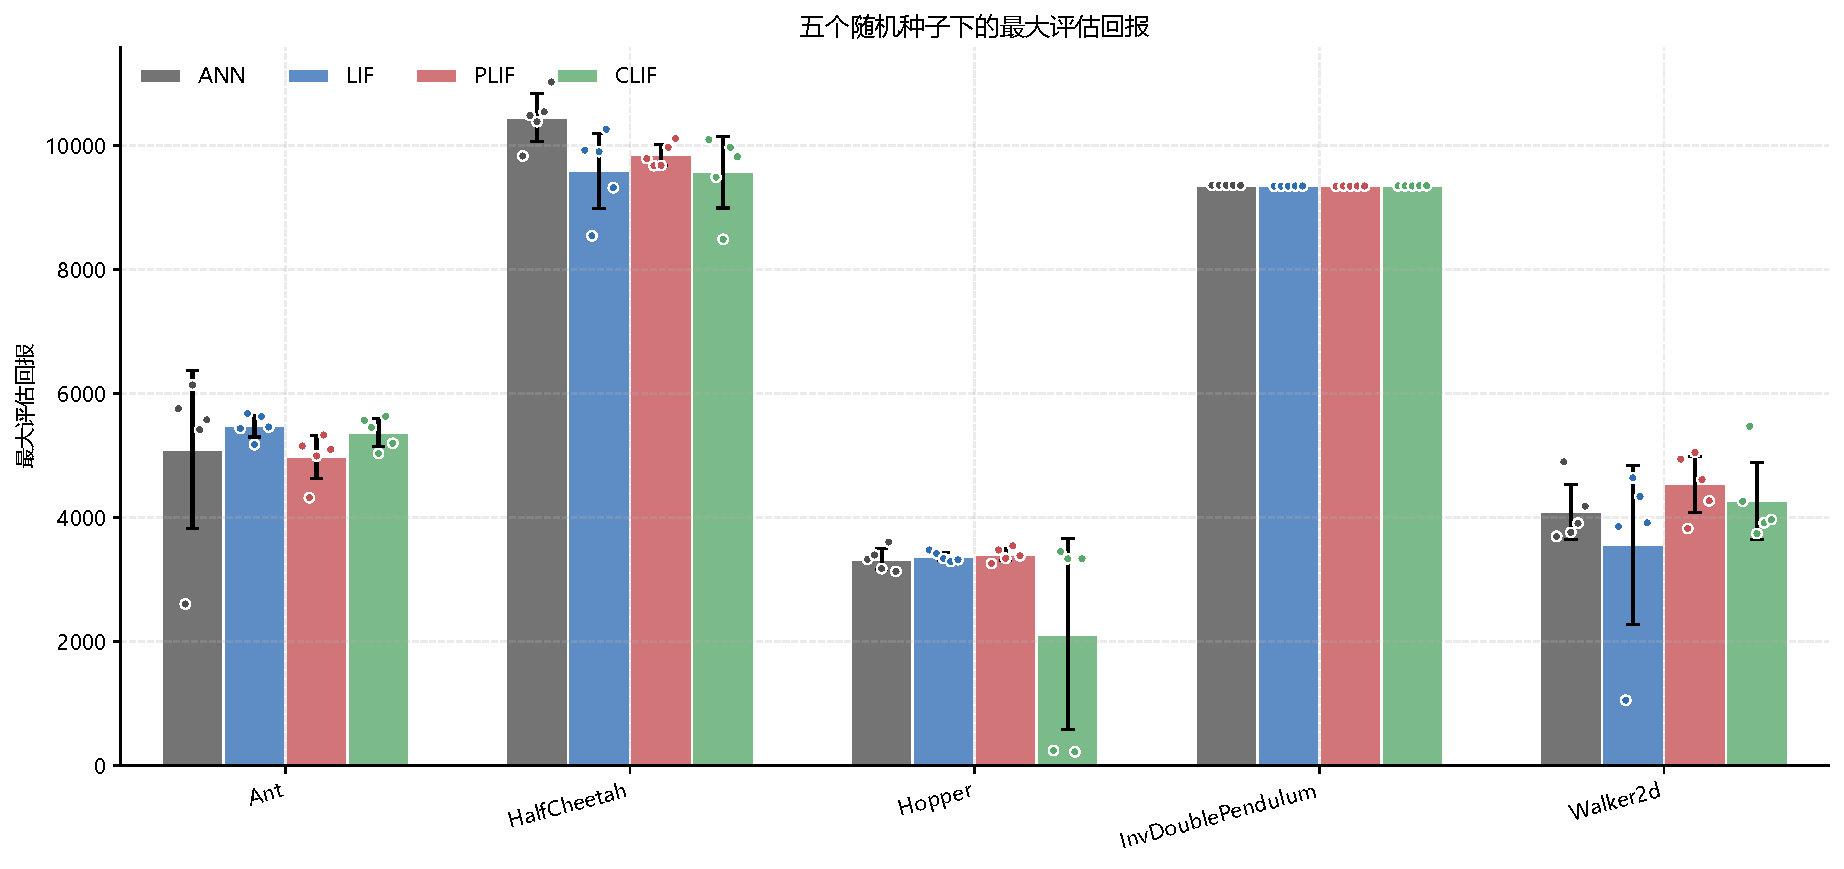
\includegraphics[width=\textwidth]{../../figures/algorithm_max_eval.pdf}
\caption{不同算法在五个 MuJoCo 环境中的最大评估回报对比}
\label{fig:algorithm-max-eval}
\end{figure}

从总体结果展示方式上看，最大评估回报能够直接反映不同方法在一次训练过程中达到过的最好策略水平，但它不能单独解释策略如何达到该水平，也不能说明失败组在训练中是否经历过梯度塌缩。因此，本文还需要结合学习曲线和 STBP 诊断指标进行后续分析。

图 \ref{fig:algorithm-learning-curves} 展示了四类方法在五个环境中的平均学习曲线。与最大评估回报相比，学习曲线能够更清楚地反映训练过程中的收敛速度、早期波动、后期稳定性以及不同随机种子之间的分化情况。对于本文关注的脉冲 actor 训练机制而言，学习曲线还可以帮助定位哪些环境和算法组合更容易出现长期低回报或早期学习停滞。

\begin{figure}[!htbp]
\centering
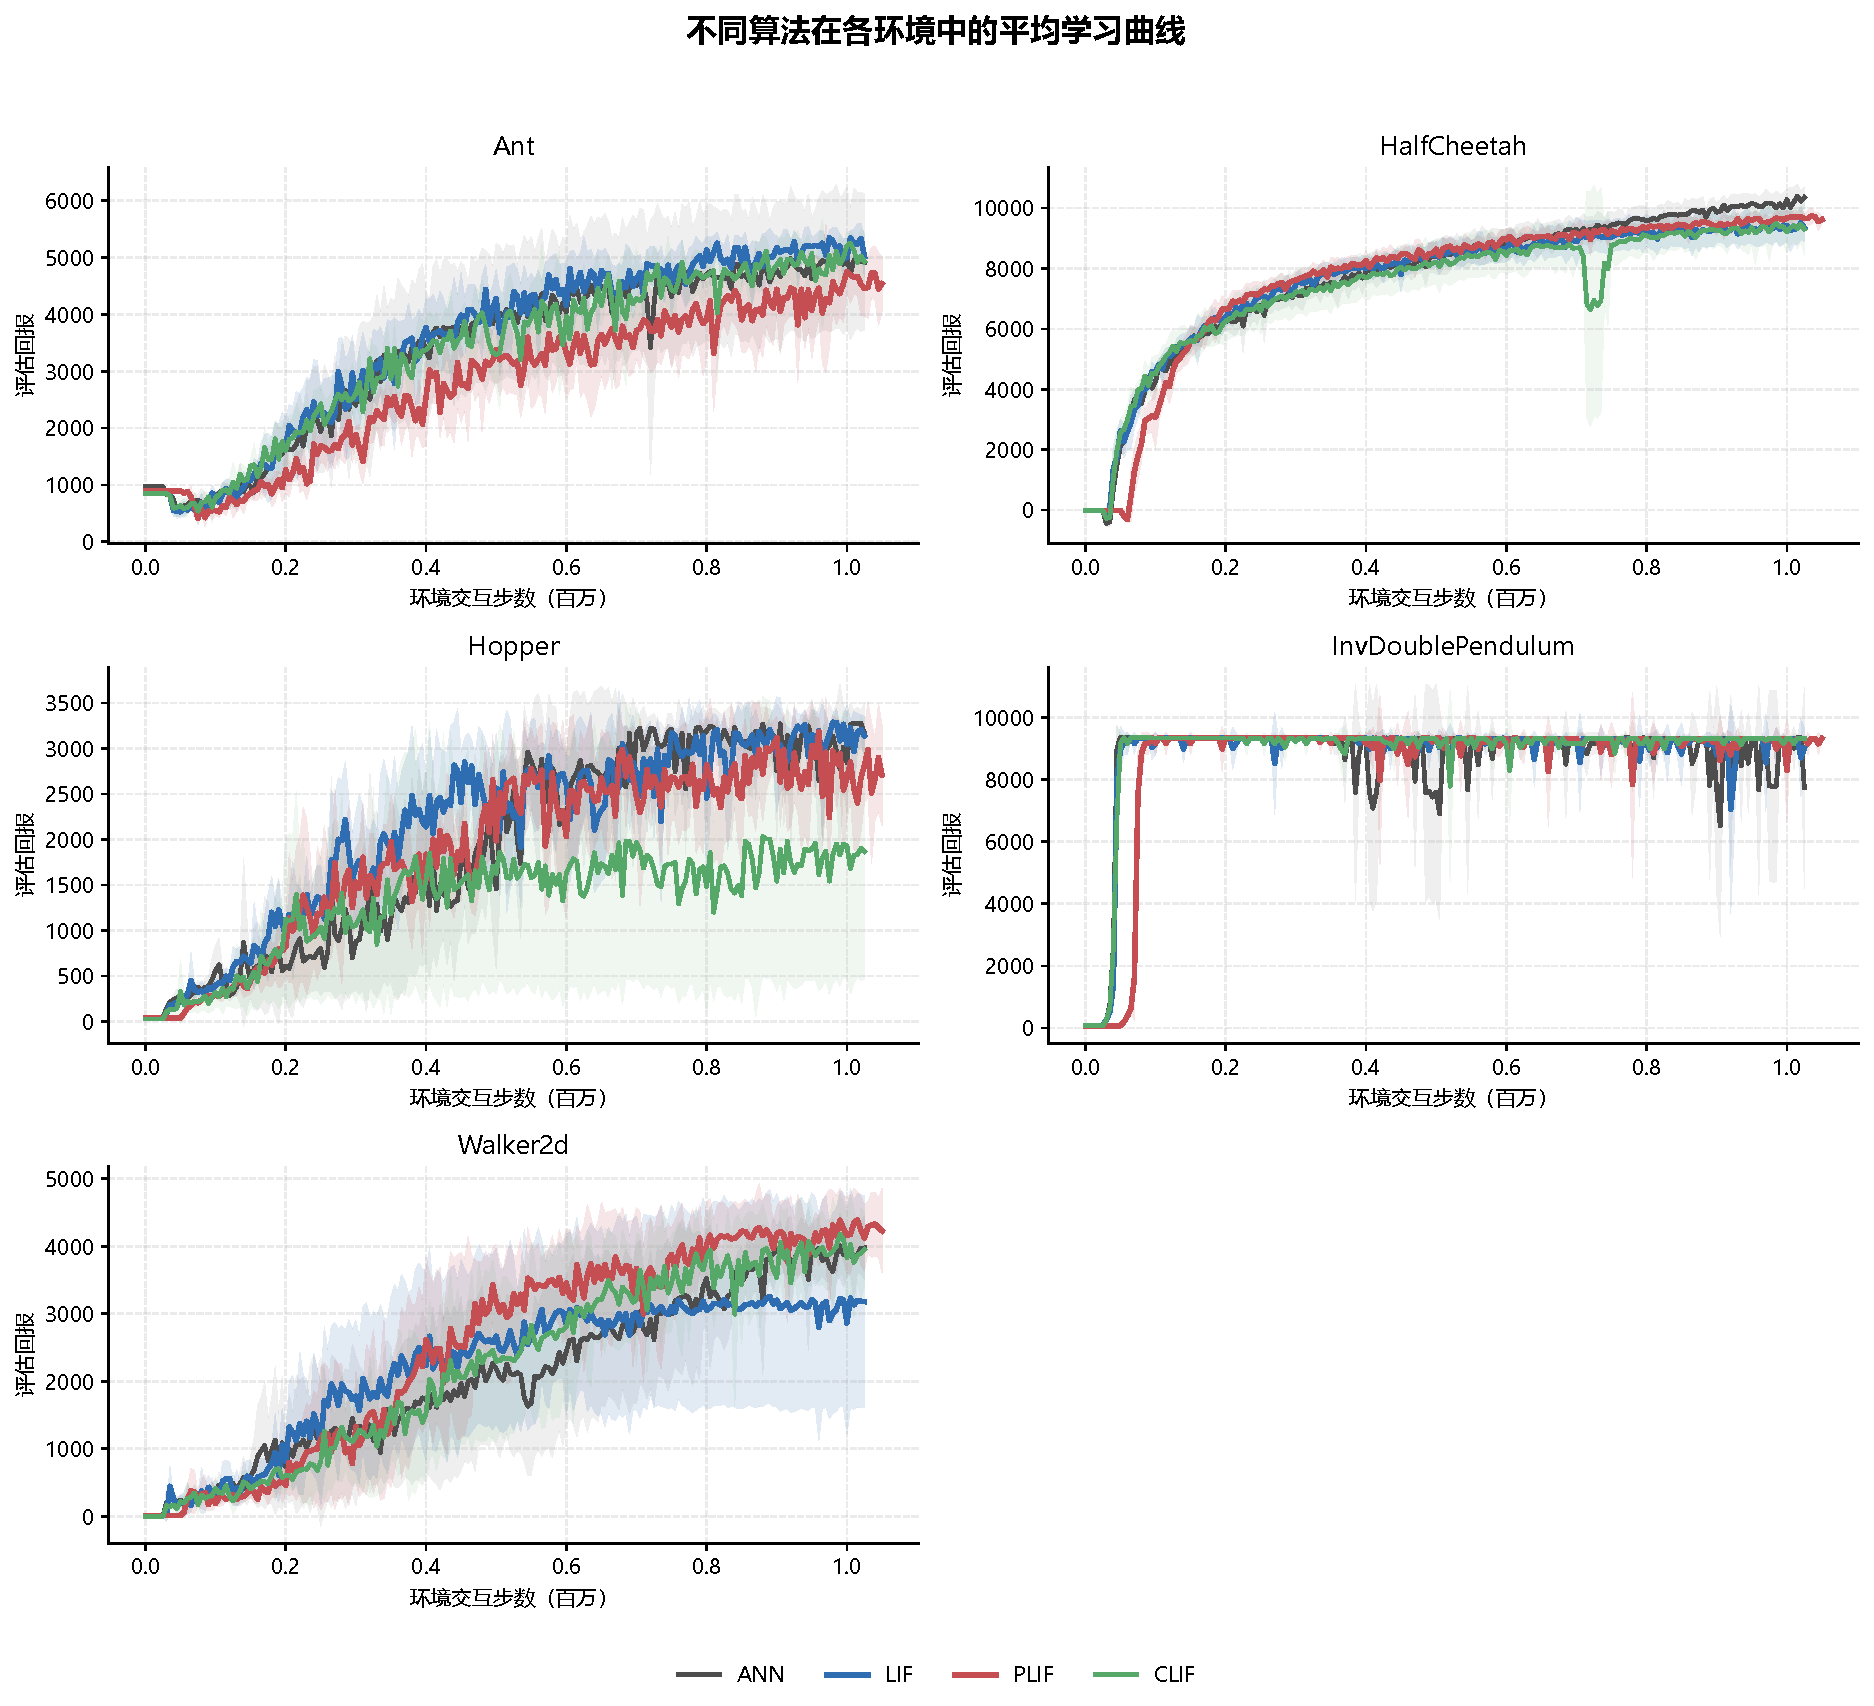
\includegraphics[width=\textwidth,height=0.82\textheight,keepaspectratio]{../../figures/algorithm_learning_curves.pdf}
\caption{不同算法在五个 MuJoCo 环境中的学习曲线对比}
\label{fig:algorithm-learning-curves}
\end{figure}

上述结果先给出四类算法的整体表现入口。接下来，本文从 Hopper-v4 中观察到的学习失败现象入手，先验证该失败现象是否能够在相同设置下复现，并进一步考察调整 actor 更新频率是否能够缓解这一问题。

\section{学习失败现象的复现与缓解}
从前述总体实验结果可以看到，Hopper-v4 是脉冲 actor 训练中较容易出现异常分化的环境之一。在默认 Proxy Target + PLIF 设置下，部分实验虽然能够持续产生动作和脉冲活动，但评估回报长期停留在较低水平，表现为明显的学习失败。为了确认该现象不是单个日志文件或偶然评估波动造成的，本文选取 Hopper-v4、随机种子 10991 作为代表性案例，对默认失败配置重复运行五次，并与只调整 \texttt{policy\_freq} 的配置进行对比。

图 \ref{fig:plif-hopper-repeat-learning-curves} 展示了两组实验的学习曲线。红色虚线对应默认失败组，主要配置为 proxy 学习率 $1\times10^{-3}$、actor 更新间隔 $2$；蓝色实线对应 actor 更新频率调整组，在保持其他主要训练设置不变的情况下，将 actor 更新间隔调整为 $4$。两组实验均使用 Hopper-v4、随机种子 10991，并各自重复运行五次。

\begin{figure}[htbp]
\centering
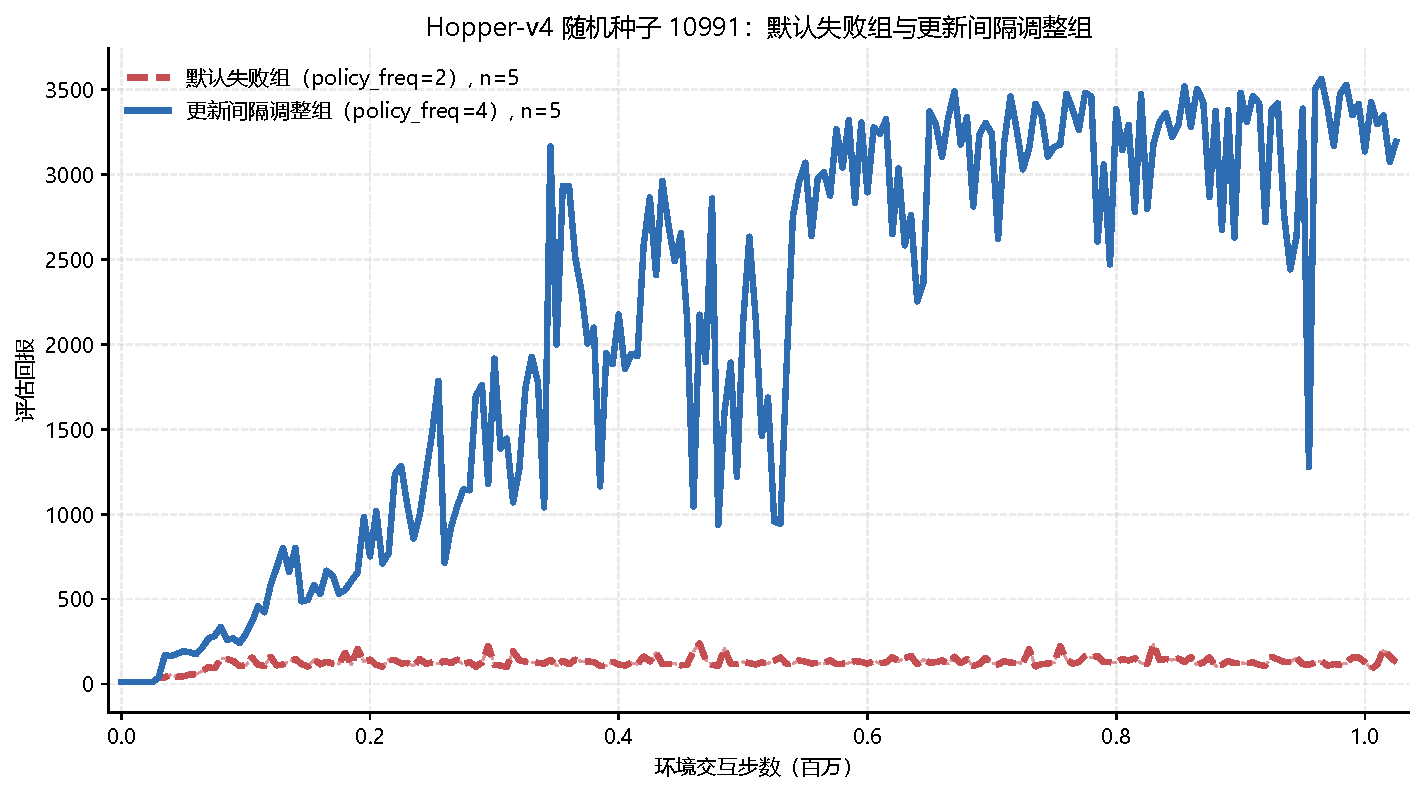
\includegraphics[width=\textwidth]{../../figures/plif_hopper_seed10991_repeat_learning_curves.pdf}
\caption{Hopper-v4 随机种子 10991 下默认失败组与 \texttt{policy\_freq} 调整组的重复运行学习曲线}
\label{fig:plif-hopper-repeat-learning-curves}
\end{figure}

结果表明，默认失败组在整个训练过程中始终停留在低回报区间，五次重复运行的最大评估回报均为 $239.393$，最终评估回报为 $129.529$。相同随机种子下，将 \texttt{policy\_freq} 从 $2$ 调整为 $4$ 后，学习曲线明显进入高回报区间，五次重复运行的最大评估回报达到 $3563.550$，最终评估回报为 $3192.666$。这说明，在当前实验设置中，Hopper-v4 上观察到的低回报停滞现象可以被稳定复现，而降低 actor 更新频率能够显著缓解该失败现象。

需要说明的是，本节中的五次重复均使用相同随机种子 10991，且当前实现下同组五条曲线完全重合。因此，该实验更适合用于说明“相同设置下失败现象和缓解现象均可复现”，而不应被解释为跨随机种子的统计显著性结论。后续分析将进一步结合 STBP 梯度信息、放电率、电流、膜电位和参数梯度，解释为什么调整 \texttt{policy\_freq} 会使训练从低回报停滞转向有效学习。

\section{STBP 梯度塌缩与放电状态诊断}
上一节已经说明，在 Hopper-v4 随机种子 10991 上，默认 PLIF 配置会稳定停留在低回报区间，而将 \texttt{policy\_freq} 从 $2$ 调整为 $4$ 后能够进入高回报区间。本节进一步从 STBP 梯度传播和放电状态两个角度解释这种差异。为保证两组实验之间具有一致的比较基础，本文重点考察两组均可稳定统计的诊断指标，包括梯度绝对值、梯度范数和放电率等。具体聚合时，先在每个训练记录点和每一层内部对 $5$ 个脉冲时间步取平均，再对同组 $5$ 次重复运行取平均。

为了说明“仍然放电”与“仍然可学习”之间的差异，可以先从单层 PLIF 神经元的反向传播路径观察梯度塌缩的来源。对于第 $l$ 层第 $t$ 个时间步，
\begin{equation}
v_t^l=\tau_l v_{t-1}^l(1-s_{t-1}^l)+I_t^l,\quad
s_t^l=H(v_t^l-V_{\mathrm{th}}).
\end{equation}
在代理梯度训练中，脉冲函数的反向传播近似为
\begin{equation}
\gamma_t^l
=
\frac{\partial s_t^l}{\partial v_t^l}
\approx
\mathbb{I}\left(|v_t^l-V_{\mathrm{th}}|<\Delta\right).
\end{equation}
因此，损失对权重的梯度可概括为
\begin{equation}
\frac{\partial \mathcal{L}}{\partial W^l}
=
\sum_t
\frac{\partial \mathcal{L}}{\partial v_t^l}
\frac{\partial v_t^l}{\partial I_t^l}
\frac{\partial I_t^l}{\partial W^l}
\propto
\sum_t
\delta_t^l (s_t^{l-1})^\top,
\end{equation}
其中 $\delta_t^l=\partial \mathcal{L}/\partial v_t^l$ 需要经过代理梯度项 $\gamma_t^l$ 以及膜电位时间递推路径继续传播。若膜电位长期落在代理梯度窗口外，则 $\gamma_t^l$ 接近零；若上一时刻频繁放电，则递推项中的 $(1-s_{t-1}^l)$ 会削弱甚至切断膜电位历史路径。此时即使前向传播仍产生大量脉冲，权重和偏置的有效梯度也可能迅速塌缩。

对于 PLIF 的可学习参数 $w_l$，更完整的理解需要显式写出时间递推关系。由于 $v_{t-1}^l$ 和 $s_{t-1}^l$ 本身也受 $w_l$ 影响，不能简单地把 $v_{t-1}^l$ 视为常数。令
\begin{equation*}
e_t^l=\frac{\partial v_t^l}{\partial w_l}
\end{equation*}
表示第 $t$ 个时间步膜电位对 PLIF 参数的敏感度，初始膜电位固定时可令初始敏感度为 $0$。对第 $l$ 层自身的 PLIF 参数而言，$I_t^l$ 不直接包含 $w_l$。由
\begin{equation*}
v_t^l=\tau_l v_{t-1}^l(1-s_{t-1}^l)+I_t^l,\quad \tau_l=\sigma(w_l)
\end{equation*}
可得如下递推形式：
\begin{equation}
e_t^l
=
v_{t-1}^l(1-s_{t-1}^l)
\tau_l(1-\tau_l)
+
\tau_l\left[(1-s_{t-1}^l)-v_{t-1}^l\gamma_{t-1}^l\right]e_{t-1}^l,
\end{equation}
其中 $\gamma_{t-1}^l$ 为上一时间步反向传播中实际采用的代理梯度。按照本文的矩形窗口近似，有 $\gamma_{t-1}^l=\mathbb{I}(|v_{t-1}^l-V_{\mathrm{th}}|<\Delta)$，用于近似脉冲函数对膜电位的真实导数。该递推式包含两类影响：第一项是 $w_l$ 通过当前时间步的 $\tau_l$ 直接改变膜电位保留项；第二项是 $w_l$ 先影响历史膜电位和历史放电，再通过 $v_{t-1}^l$ 与 $(1-s_{t-1}^l)$ 传递到当前膜电位。最终，PLIF 参数的梯度由所有时间步的贡献累积得到：
\begin{equation}
\frac{\partial \mathcal{L}}{\partial w_l}
=
\sum_t
\frac{\partial \mathcal{L}}{\partial v_t^l}
e_t^l.
\end{equation}
因此，当膜电位长期偏离代理梯度窗口时，$\gamma_{t-1}^l$ 以及 $\partial \mathcal{L}/\partial v_t^l$ 都可能变小；当频繁放电使 $(1-s_{t-1}^l)$ 经常接近零时，历史膜电位路径也会被削弱。此时 PLIF 时间常数虽然是可学习参数，也无法继续获得有效更新。后续的梯度和放电率诊断正是围绕这一反向传播路径展开。

为便于理解后续两组诊断图，表 \ref{tab:stbp-diagnostic-metrics} 汇总了本节使用的主要指标。整体上，梯度指标用于判断 actor 是否仍能获得反向学习信号，放电率指标用于判断前向脉冲活动是否沉默或饱和。

\begin{table}[H]
\centering
\caption{Hopper-v4 失败机制分析中的诊断指标说明}
\label{tab:stbp-diagnostic-metrics}
\zihao{5}
\setlength{\tabcolsep}{3pt}
\begin{tabular}{p{0.24\textwidth}p{0.28\textwidth}p{0.38\textwidth}}
\toprule
\textbf{指标} & \textbf{计算形式} & \textbf{含义与机制解释} \\
\midrule
电流梯度 & $\left|\partial\mathcal{L}/\partial I_t\right|$ & 损失对神经元输入电流的梯度幅值，用于判断 STBP 误差信号是否能够传回当前层。 \\
时间步权重梯度 & $\|\nabla_{W,t}\mathcal{L}\|_2$ & 单个脉冲时间步中权重接收到的梯度强度，用于观察时间展开路径中的梯度是否仍然存在。 \\
参数级权重梯度 & $\|\nabla_W\mathcal{L}\|_2$ & 聚合到实际网络参数后的权重梯度范数，直接反映优化器能否继续更新 actor 权重。 \\
PLIF 时间常数梯度 & $\left|\partial\mathcal{L}/\partial w_l\right|$ & 可学习时间常数参数的梯度幅值，用于判断 PLIF 时间尺度是否仍能被策略损失调整。 \\
阈值前放电率 & $\mathbb{E}[s_t^{l-1}]$ & 进入当前层的上一层脉冲活动比例，用于衡量当前层输入脉冲是否充足。 \\
阈值后放电率 & $\mathbb{E}[s_t^l]$ & 当前层输出脉冲比例，用于判断该层是否处于沉默、稀疏放电或高放电状态。 \\
\bottomrule
\end{tabular}
\end{table}

图 \ref{fig:plif-stbp-gradient-collapse} 给出了三层 actor 在训练过程中的 STBP 梯度变化。为了同时显示早期小梯度和后期零梯度，纵轴采用对数坐标，精确为零的值在图中用 $10^{-12}$ 显示。从图中可以看到，默认失败组的电流梯度、逐时间步权重梯度、参数级权重梯度以及时间常数梯度都在训练早期后迅速塌缩。五次重复运行中，最后一次非零梯度均出现在第 $19800$ 次训练迭代，之后直到第 $1000000$ 次训练迭代均不再记录到非零梯度。相反，\texttt{policy\_freq}=4 组直到训练末尾仍保持非零梯度，说明成功组的 actor 参数和 PLIF 时间常数仍能从策略损失获得学习信号。

\begin{figure}[H]
\centering
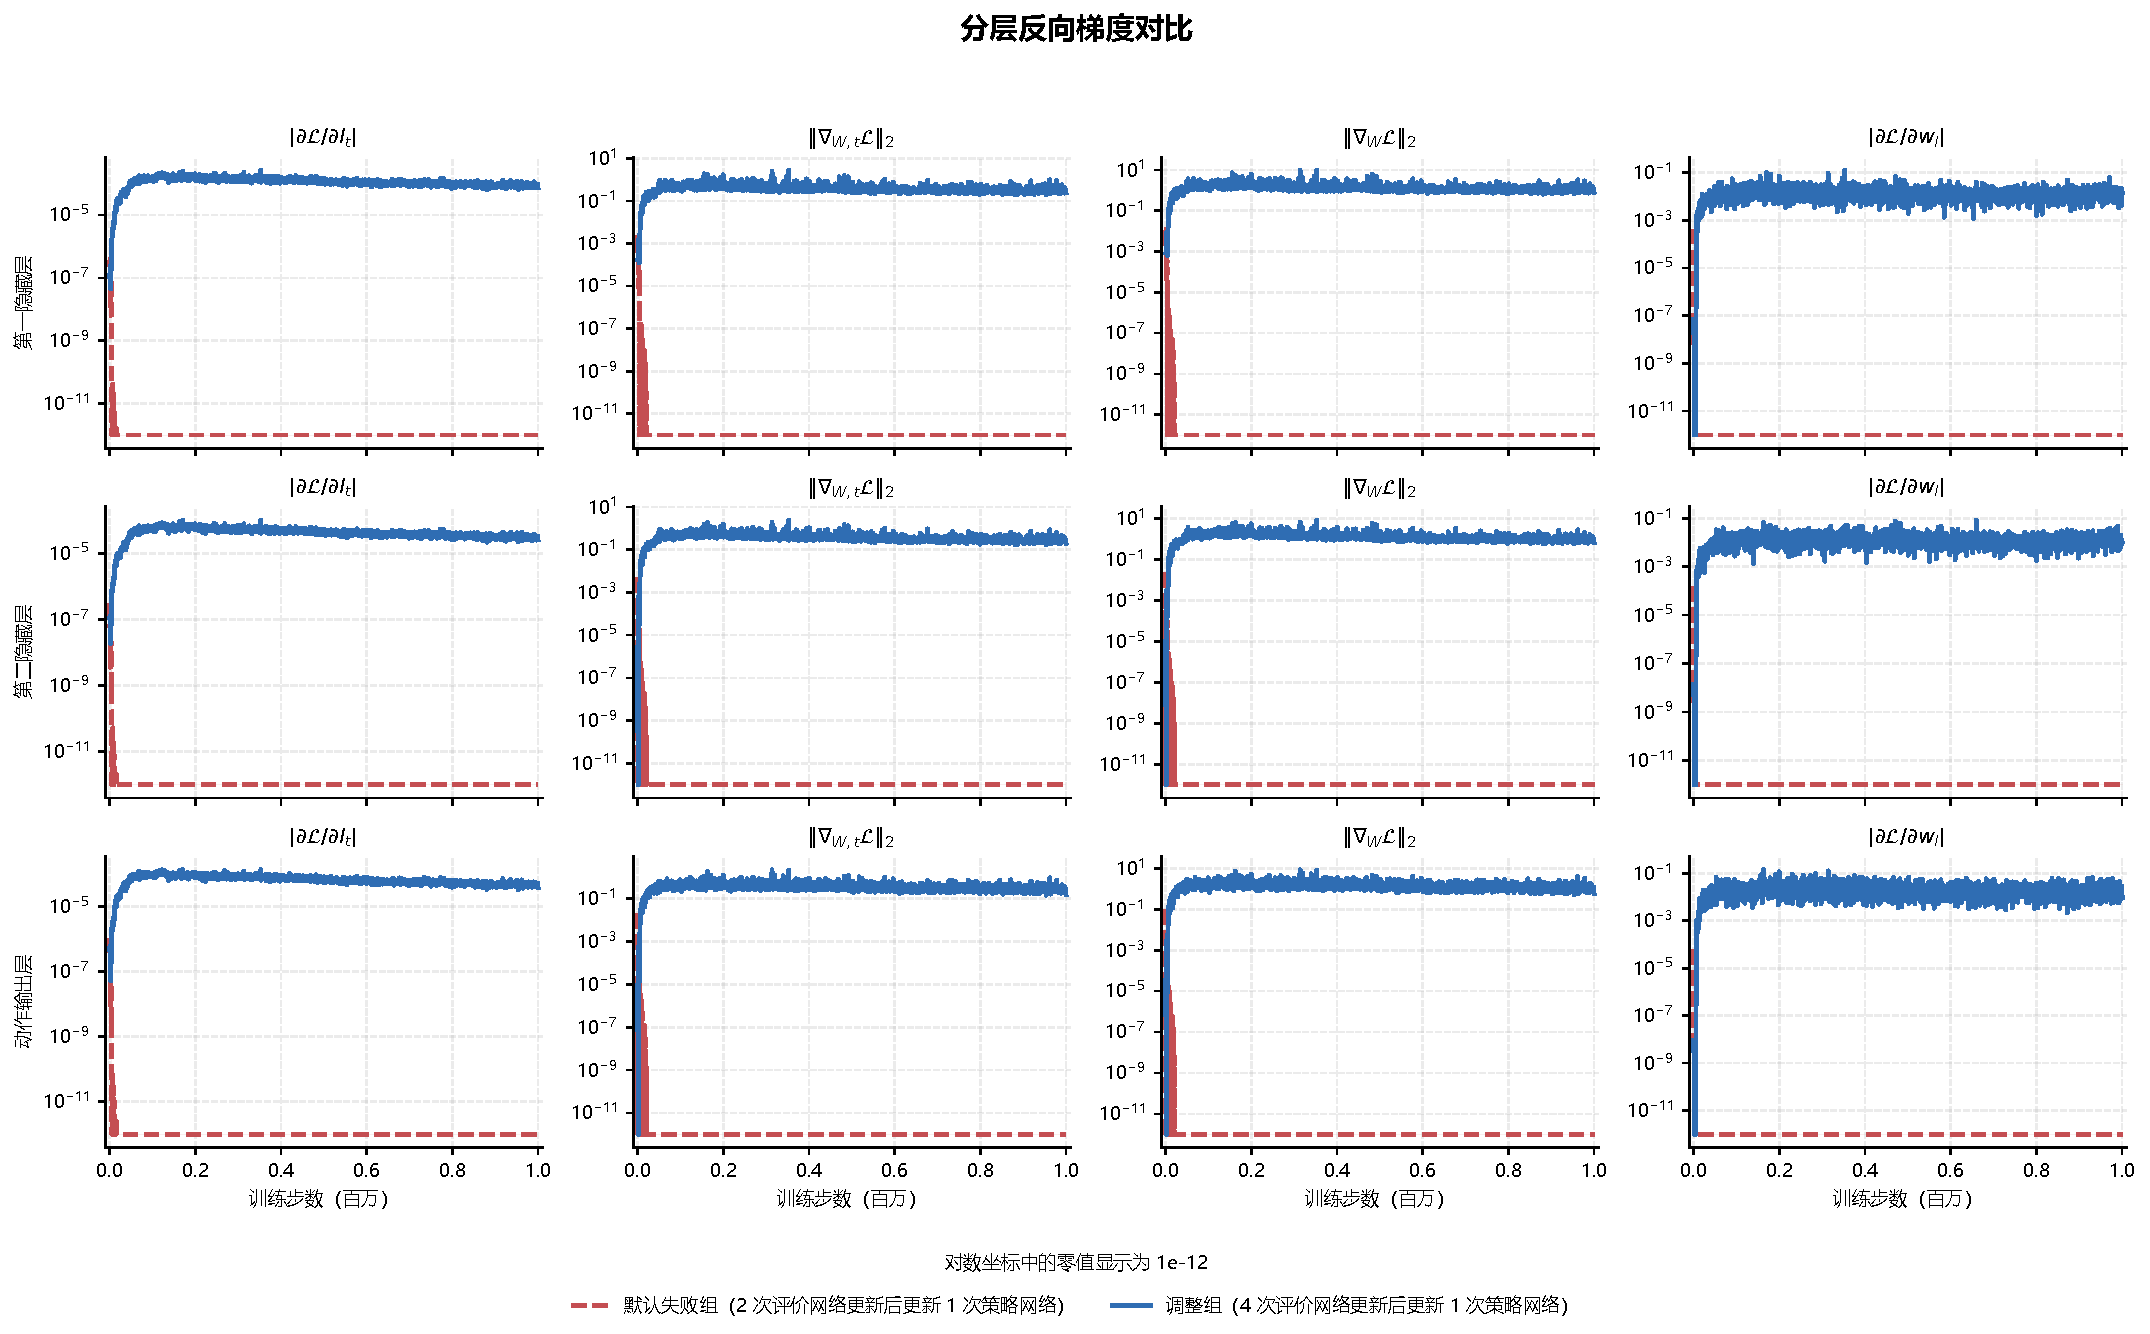
\includegraphics[width=\textwidth,height=0.72\textheight,keepaspectratio]{../../figures/plif_stbp_gradient_collapse.pdf}
\caption{Hopper-v4 随机种子 10991 下默认失败组与 actor 更新间隔调整组的分层 STBP 梯度对比。每条曲线先对 $5$ 个脉冲时间步聚合，再对 $5$ 次重复运行取平均；对数坐标中精确零值以 $10^{-12}$ 显示。}
\label{fig:plif-stbp-gradient-collapse}
\end{figure}

梯度消失并不等价于网络没有放电。图 \ref{fig:plif-stbp-spike-rates} 展示了相同两组实验的阈值前放电率与阈值后放电率。失败组在训练后期仍然保持明显的脉冲活动：第一隐藏层、第二隐藏层和动作输出层的后期平均阈值后放电率分别约为 $0.650$、$0.505$ 和 $0.566$。这说明失败组并不是进入了脉冲沉默状态，网络前向传播仍在产生大量脉冲和连续动作。与之相比，\texttt{policy\_freq}=4 成功组的隐藏层更稀疏，后期第一隐藏层与第二隐藏层的阈值后放电率约为 $0.211$ 和 $0.356$，但动作输出层仍保持约 $0.532$ 的放电率。这种差异说明，仅观察放电率不足以判断 actor 是否仍能学习；高放电率也可能对应饱和或低效的反向传播状态。

\begin{figure}[H]
\centering
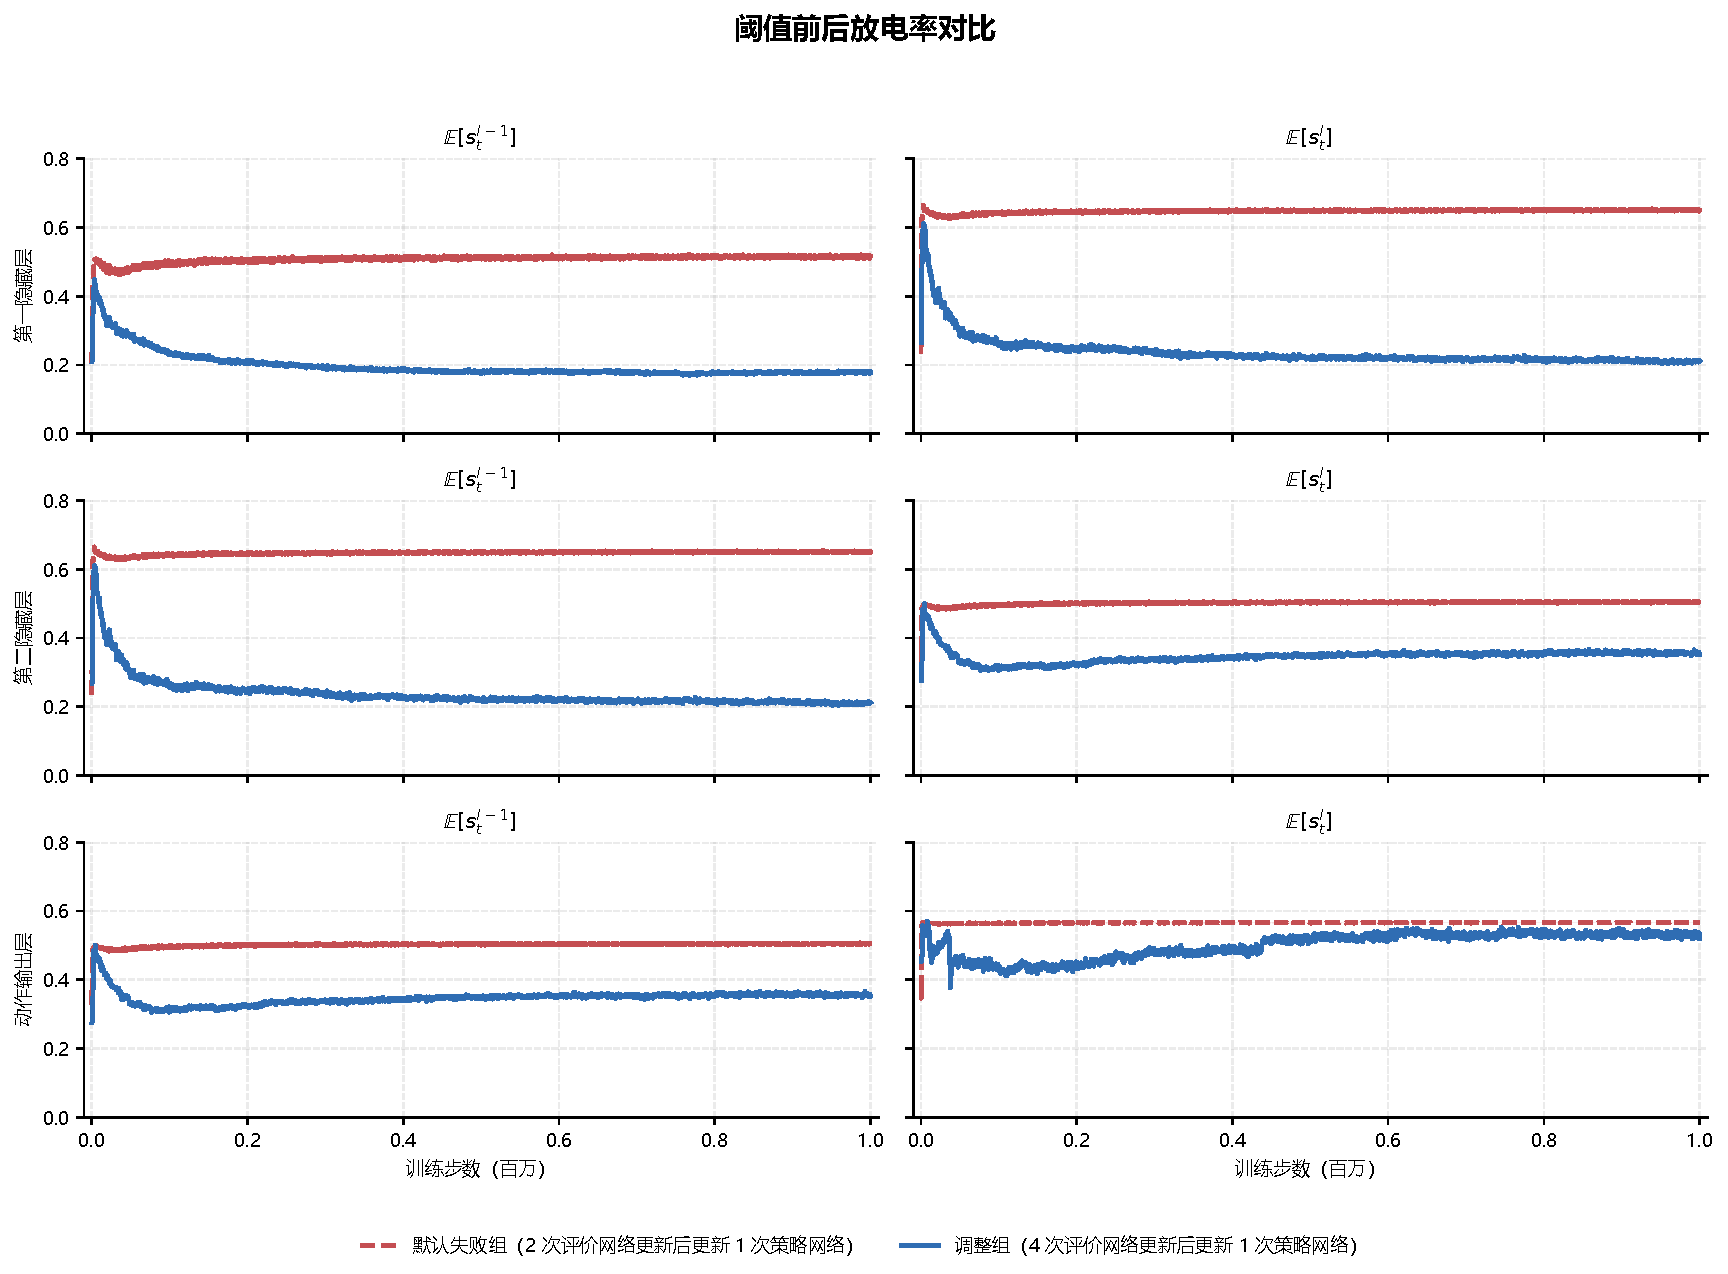
\includegraphics[width=\textwidth,height=0.70\textheight,keepaspectratio]{../../figures/plif_stbp_spike_rates.pdf}
\caption{Hopper-v4 随机种子 10991 下默认失败组与 actor 更新间隔调整组的阈值前放电率与阈值后放电率对比。失败组后期仍保持较高阈值后放电率，说明低回报停滞不是由脉冲沉默直接造成。}
\label{fig:plif-stbp-spike-rates}
\end{figure}

综合来看，默认失败组的关键问题不是前向脉冲完全消失，而是在仍然保持较高放电率的同时，有效 STBP 梯度已经塌缩。一方面，频繁放电会通过重置项 $(1-s_{t-1})$ 削弱膜电位沿时间维度传递的路径；另一方面，图 \ref{fig:plif-stbp-gradient-collapse} 中的电流梯度、权重梯度和 PLIF 时间常数梯度直接表明失败组后期已经无法继续获得有效反向学习信号。此时权重、偏置和 PLIF 时间常数的梯度都会趋近于零，PLIF 额外提供的可学习时间常数也无法继续调整。相比之下，\texttt{policy\_freq}=4 组在隐藏层保持更稀疏的放电，并持续保留非零 STBP 梯度，因此 actor 能够继续通过 critic 提供的策略损失更新参数，最终进入高回报区间。

需要再次强调，本文中的五次重复运行使用相同随机种子，因此本节结论主要说明相同设置下的机制可复现性，而不是跨随机种子的统计显著性。不过，这一对照已经足以支持本文的核心机制判断：在当前 Proxy Target + PLIF 训练中，失败组的低回报停滞更接近“仍然放电但梯度塌缩”的状态，而不是简单的脉冲沉默或动作输出缺失。

\FloatBarrier

\section{PLIF 时间常数的层间演化}
上一节说明了成功组能够持续保留非零 STBP 梯度。本节进一步考察 PLIF 的可学习时间常数在训练中具体学到了什么。图 \ref{fig:plif-tau-curves} 展示了常规 PT-PLIF 实验中不同环境下三层 PLIF 时间常数的平均演化曲线。整体上，隐藏层时间常数往往从初始化附近逐渐升高，而动作输出层时间常数的变化更保守，在 Hopper-v4、HalfCheetah-v4 和 Walker2d-v4 中甚至出现后期下降。这说明 PLIF 并不是在所有层上无差别地增大时间常数，而是呈现出明显的层间分化：隐藏层更倾向于学习较长的膜电位保留时间，动作输出层则更直接服务于动作种群的读出，对时间常数的需求可能更短。

\begin{figure}[!htbp]
\centering
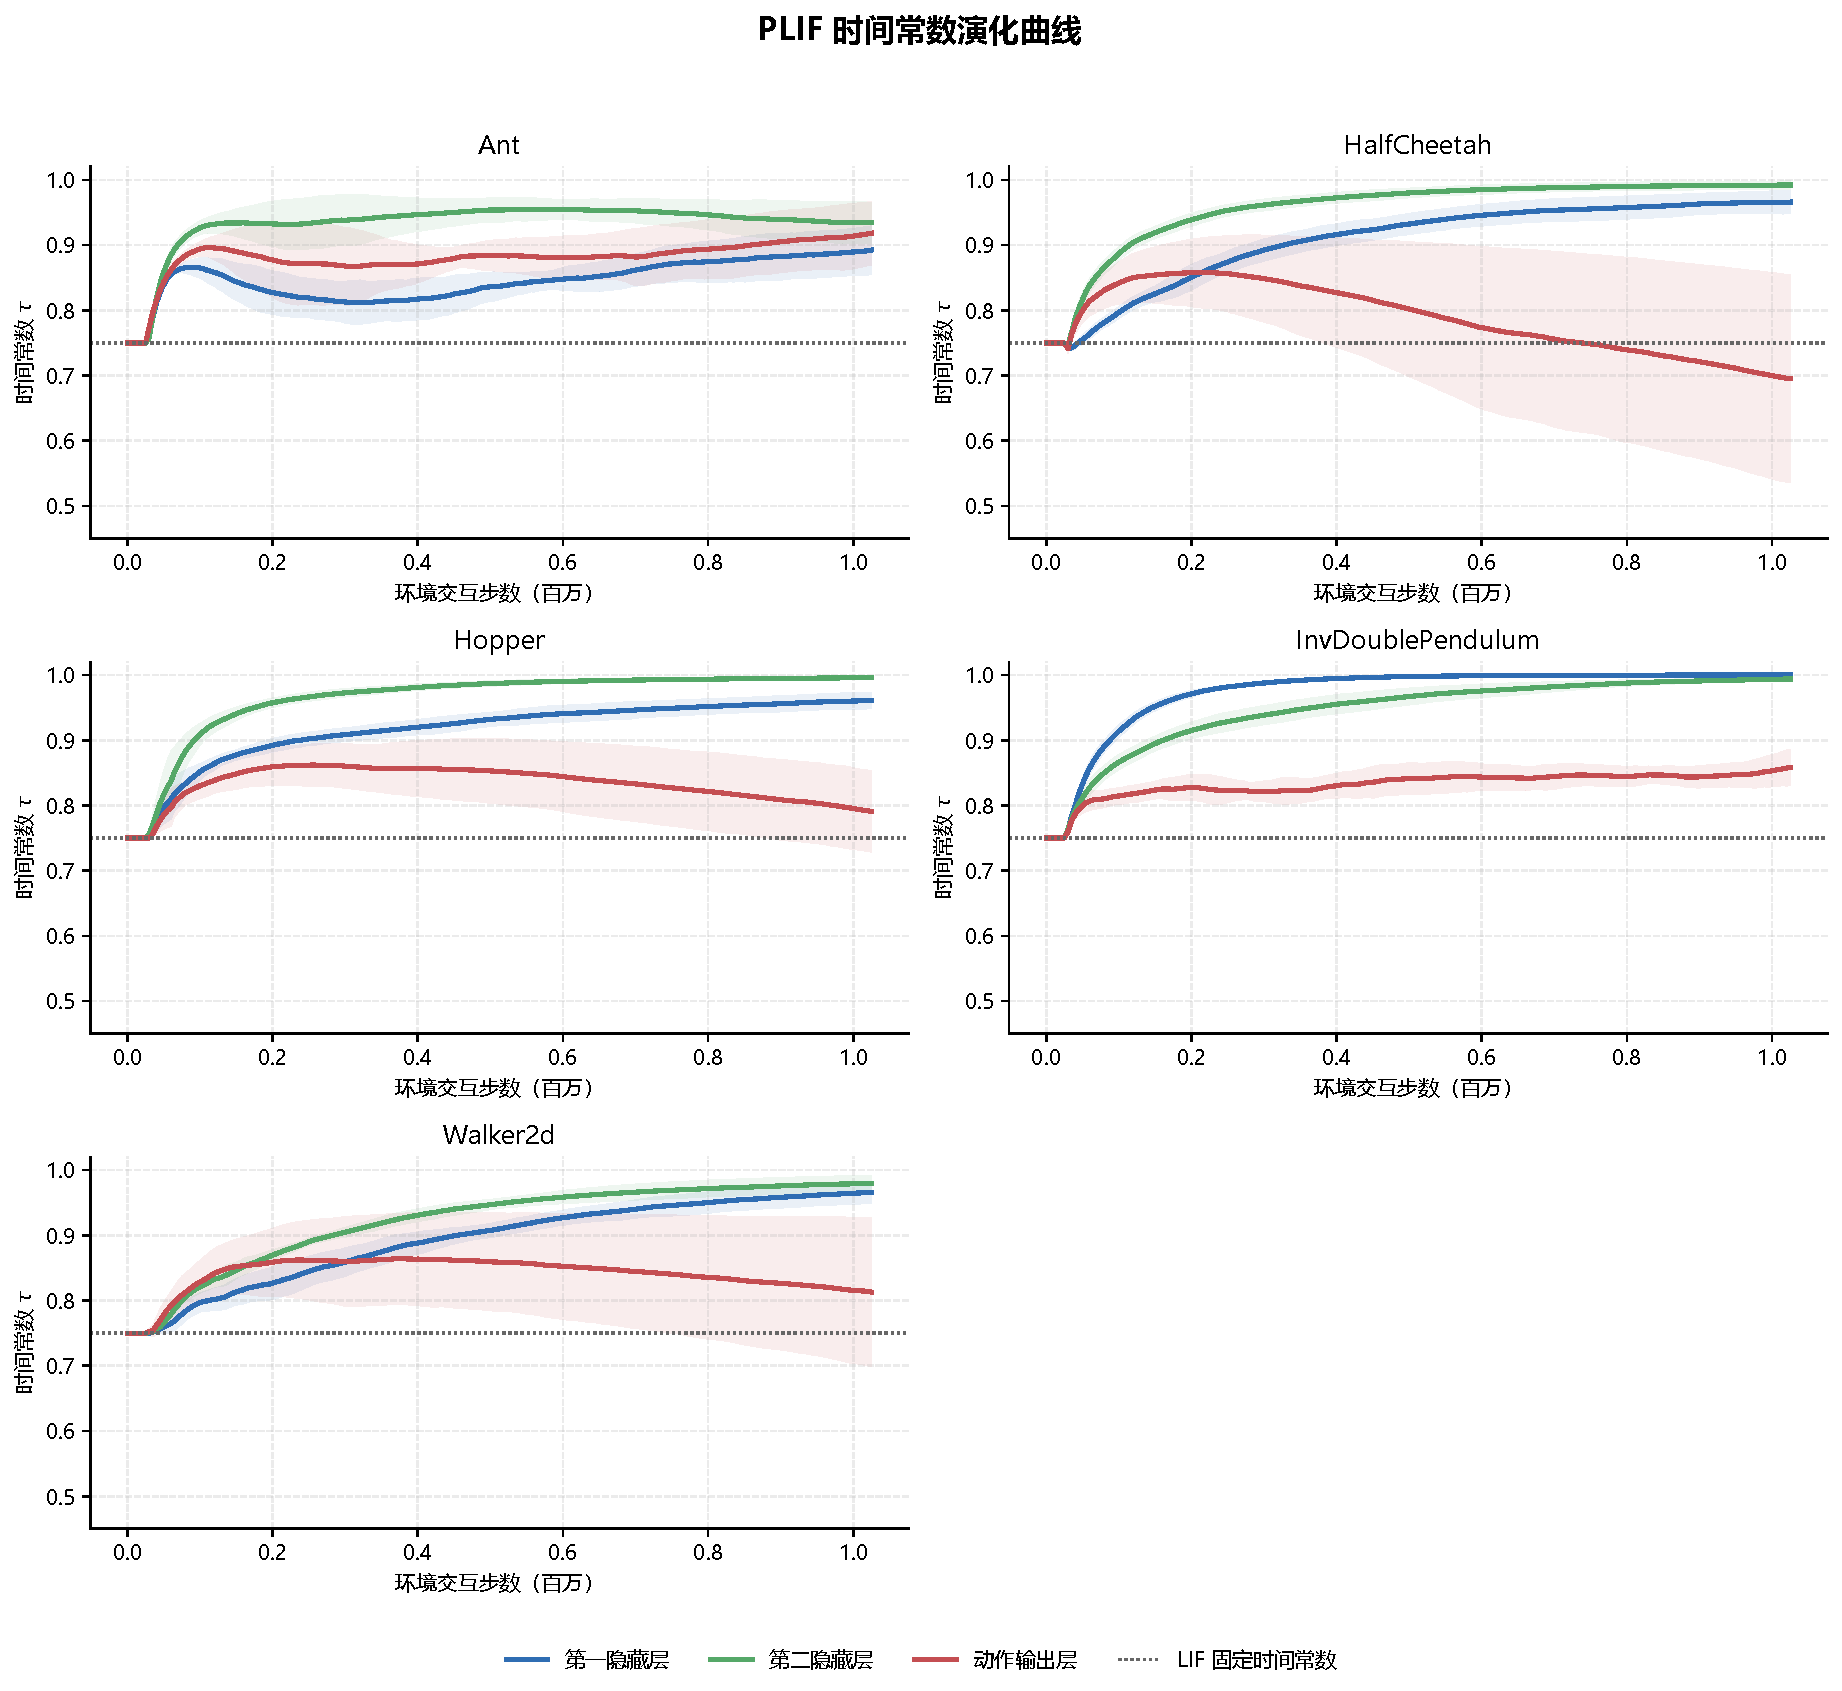
\includegraphics[width=\textwidth,height=0.82\textheight,keepaspectratio]{../../figures/plif_tau_curves.pdf}
\caption{常规 PT-PLIF 实验中不同环境的 PLIF 时间常数演化曲线。蓝色和绿色分别表示两层隐藏层 PLIF 神经元模块，红色表示动作输出层，灰色虚线表示与 LIF 对齐的固定初始值 $0.75$。}
\label{fig:plif-tau-curves}
\end{figure}

为了结合前文 Hopper-v4 的成功对照机制，本文进一步统计 actor 更新频率调整组的 PLIF 时间常数演化情况。该组中第一隐藏层、第二隐藏层和动作输出层的时间常数分别从约 $0.7507$、$0.7504$ 和 $0.7506$ 演化到 $0.9566$、$0.9943$ 和 $0.6929$。因此，在 \texttt{policy\_freq}=4 的成功组中，被显著推高的是隐藏层时间常数，而不是动作输出层时间常数。

有效保留项来自 PLIF 膜电位递推式中历史膜电位的系数。对于第 $l$ 层第 $t$ 个脉冲时间步，有
\[
v_t^l=\tau_l v_{t-1}^l(1-s_{t-1}^l)+I_t^l
=\underbrace{\tau_l(1-s_{t-1}^l)}_{\text{历史膜电位保留系数}}v_{t-1}^l+I_t^l.
\]
因此，上一时刻膜电位能否进入当前时刻同时受到时间常数 $\tau_l$ 和上一时刻放电重置项 $(1-s_{t-1}^l)$ 的影响。若上一时刻已经放电，则 $s_{t-1}^l=1$，历史膜电位项被切断；若未放电，则该路径按比例 $\tau_l$ 保留。对同一层的样本、神经元和脉冲时间步取平均时，可将有效保留项写为
\[
R_l=\mathbb{E}[\tau_l(1-s_{t-1}^l)].
\]
由于本文代码中每个 PLIF 层共享一个标量时间常数，表 \ref{tab:policy-freq-tau} 中进一步使用同层阈值后平均放电率 $\bar{s}$ 近似该平均量，即 $R_l\approx\tau_l(1-\bar{s})$。表中统计对象为前文 Hopper-v4 随机种子 10991 下的 actor 更新频率调整组，即 \texttt{policy\_freq}=4 的五次重复运行。具体统计时，时间常数的初始值和最终值分别取该组记录的首次与末次观测；早期窗口定义为 \texttt{train\_it}$\le 20000$，后期窗口定义为 \texttt{train\_it}$\ge 700000$。表中有效保留项按对应窗口内的平均时间常数和平均阈值后放电率计算，因此反映的是训练阶段窗口平均意义下的膜电位保留能力。

\begin{table}[htbp]
\centering
\caption{actor 更新频率调整组中 PLIF 时间常数、放电率与有效保留项的变化}
\label{tab:policy-freq-tau}
\zihao{5}
\setlength{\tabcolsep}{4pt}
\begin{tabular}{lcccccc}
\toprule
\textbf{层} & \multicolumn{2}{c}{\textbf{$\tau_l$}} & \multicolumn{2}{c}{\textbf{$\bar{s}$}} & \multicolumn{2}{c}{\textbf{$\tau_l(1-\bar{s})$}} \\
\cmidrule(lr){2-3}\cmidrule(lr){4-5}\cmidrule(lr){6-7}
 & \textbf{初始} & \textbf{最终} & \textbf{早期} & \textbf{后期} & \textbf{早期} & \textbf{后期} \\
\midrule
第一隐藏层 & 0.7507 & 0.9566 & 0.4838 & 0.2143 & 0.392 & 0.747 \\
第二隐藏层 & 0.7504 & 0.9943 & 0.4347 & 0.3559 & 0.430 & 0.638 \\
动作输出层 & 0.7506 & 0.6929 & 0.5080 & 0.5321 & 0.372 & 0.338 \\
\bottomrule
\end{tabular}
\end{table}

表 \ref{tab:policy-freq-tau} 中，$\bar{s}$ 表示同层阈值后放电率的平均值，$\tau_l(1-\bar{s})$ 可理解为一个近似的有效膜电位保留项。对于第一隐藏层，该值从早期约 $0.392$ 提高到后期约 $0.747$；对于第二隐藏层，该值从约 $0.430$ 提高到约 $0.638$。这表明成功组并不是通过提高隐藏层放电率来获得更强表示能力，相反，隐藏层阈值后放电率从早期较高水平下降到更稀疏的状态，而时间常数的升高增强了未放电路径上的膜电位保留能力。换言之，成功组学到的是一种“稀疏放电 + 长时间常数”的隐藏层表示方式：较低放电率减少重置项 $(1-s_{t-1}^l)$ 对历史路径的切断，较高时间常数则保留跨时间步的亚阈值信息。

从参数更新方向看，actor 更新频率调整组中的隐藏层 PLIF 参数在训练后期总体表现为提高时间常数的趋势。由于 $\tau_l=\sigma(w_l)$ 是关于 $w_l$ 的单调递增函数，$w_l$ 的增大对应更强的膜电位保留能力。相比之下，动作输出层并未呈现同步增大趋势，最终时间常数降至约 $0.6929$。这一结果说明，PLIF 时间常数的变化受到策略损失和层功能差异的共同影响，体现为层间自适应调节，而不是所有层同时增大的参数漂移。

综合来看，PLIF 在成功组中的作用可以解释为：隐藏层通过增大时间常数保留更长时间尺度的状态编码信息，同时通过较低放电率减少频繁重置对时间路径的破坏；动作输出层则不必同步增大时间常数，而是保持更短的动作读出时间尺度。这一现象也解释了为什么仅比较 PLIF 与 LIF 的最终回报不足以揭示 PLIF 的作用，必须结合时间常数演化、放电率和 STBP 梯度共同分析其训练机制。

\FloatBarrier

\section{LIF 与 PLIF 成功机制的近似等价性分析}
前文以 Hopper-v4 中 PLIF 默认失败组与 actor 更新间隔调整组为代表案例，分析了放电状态、STBP 梯度和时间常数演化在低回报停滞与训练恢复中的作用。为进一步判断 PLIF 是否使成功训练后的脉冲 actor 形成不同于 LIF 的内部机制，本节对额外整理的 PT-LIF 与 PT-PLIF 成功训练实验进行配对诊断。该分析不再以最终回报作为唯一比较对象，而是将训练后期的神经状态和反向梯度指标作为机制层面的比较依据，检验二者是否沿着相近的前向动力学和反向梯度路径完成学习。

实验样本由五个 MuJoCo 连续控制环境和三个随机种子下的 PT-LIF、PT-PLIF 成功训练记录构成。本文将训练迭代步数不小于 $900000$ 的 STBP 诊断记录作为训练后期样本，并以环境、随机种子和网络层为索引构造 LIF--PLIF 配对样本。对于每一个配对样本，本文先在同一网络层内对脉冲时间步和训练后期记录取平均，再分别得到 LIF 与 PLIF 的机制诊断值。该处理能够降低单次记录的随机波动，使比较重点集中于成功训练后形成的相对稳定内部状态。

为避免将图中的相关性解释为抽象统计量，表 \ref{tab:success-mechanism-metrics} 给出了本节使用的九个诊断指标定义。表中 $s_t^l$ 表示第 $l$ 层第 $t$ 个脉冲时间步的输出脉冲，$I_t^l$ 表示突触电流，$v_t^l$ 表示膜电位，$V_{\mathrm{th}}=0.5$ 为脉冲阈值，$\Delta=0.5$ 为矩形代理梯度窗口宽度。对于 LIF，$\tau_l$ 为固定保留系数 $0.75$；对于 PLIF，$\tau_l=\sigma(w_l)$ 为可学习时间常数。除动作梯度范数外，表中指标均先在批量样本、神经元或动作种群维度上统计，再在绘图时对脉冲时间步和训练后期记录取平均。

\begin{table}[htbp]
\centering
\caption{LIF 与 PLIF 成功机制配对分析中的诊断指标定义}
\label{tab:success-mechanism-metrics}
\zihao{5}
\setlength{\tabcolsep}{3pt}
\begin{tabular}{p{0.20\textwidth}p{0.38\textwidth}p{0.34\textwidth}}
\toprule
\textbf{指标} & \textbf{计算含义} & \textbf{机制解释} \\
\midrule
层输出放电率 & $\mathbb{E}[s_t^l]$ & 判断前向脉冲活动是否稀疏或饱和。 \\
突触电流幅值 & $\mathbb{E}[|I_t^l|]$ & 刻画输入到神经元的驱动强度。 \\
膜电位标准差 & $\mathrm{Std}(v_t^l)$ & 衡量膜电位分布尺度。 \\
电流梯度强度 & $\mathbb{E}[|\partial \mathcal{L}/\partial I_t^l|]$ & 表示电流端 STBP 梯度强度，用于判断该层是否仍能获得学习信号。 \\
代理梯度窗口占比 & $\mathbb{E}[\mathbb{I}(|v_t^l-V_{\mathrm{th}}|<\Delta)]$ & 表示膜电位落入有效代理梯度区域的比例。 \\
有效保留系数 & $\mathbb{E}[\tau_l(1-s_{t-1}^l)]$ & 同时受到时间常数和上一时刻重置项影响。 \\
真实保留电压幅值 & $\mathbb{E}[|v_{t-1}^l\tau_l(1-s_{t-1}^l)|]$ & 表示历史膜电位实际贡献到当前膜电位的强度。 \\
非零电流梯度占比 & $\mathbb{E}[\mathbb{I}(\partial \mathcal{L}/\partial I_t^l\ne 0)]$ & 衡量反向学习信号覆盖到多少神经元状态。 \\
动作梯度范数 & $\|\partial \mathcal{L}/\partial a\|_2$ & 反映 critic 传回 actor 输出端的策略更新强度。 \\
\bottomrule
\end{tabular}
\end{table}
\FloatBarrier

图 \ref{fig:lif-plif-success-mechanism-paired} 给出了九类代表性指标的 LIF--PLIF 配对散点图。其中，放电率、电流幅值、膜电位标准差和电流梯度绝对值属于前文已经使用的诊断指标；代理梯度窗口占比、有效保留项、真实保留电压、非零电流梯度占比和动作梯度范数来自进一步记录的机制诊断字段。虚线表示 $y=x$。如果 PLIF 在成功训练后形成了与 LIF 显著不同的机制状态，则配对点应当在多个指标上系统偏离 $y=x$，或者呈现较低的配对相关性；相反，若二者主要共享相近的训练动力学，则不同环境、随机种子和网络层之间的相对关系应当保持一致。

\begin{figure}[!htbp]
\centering
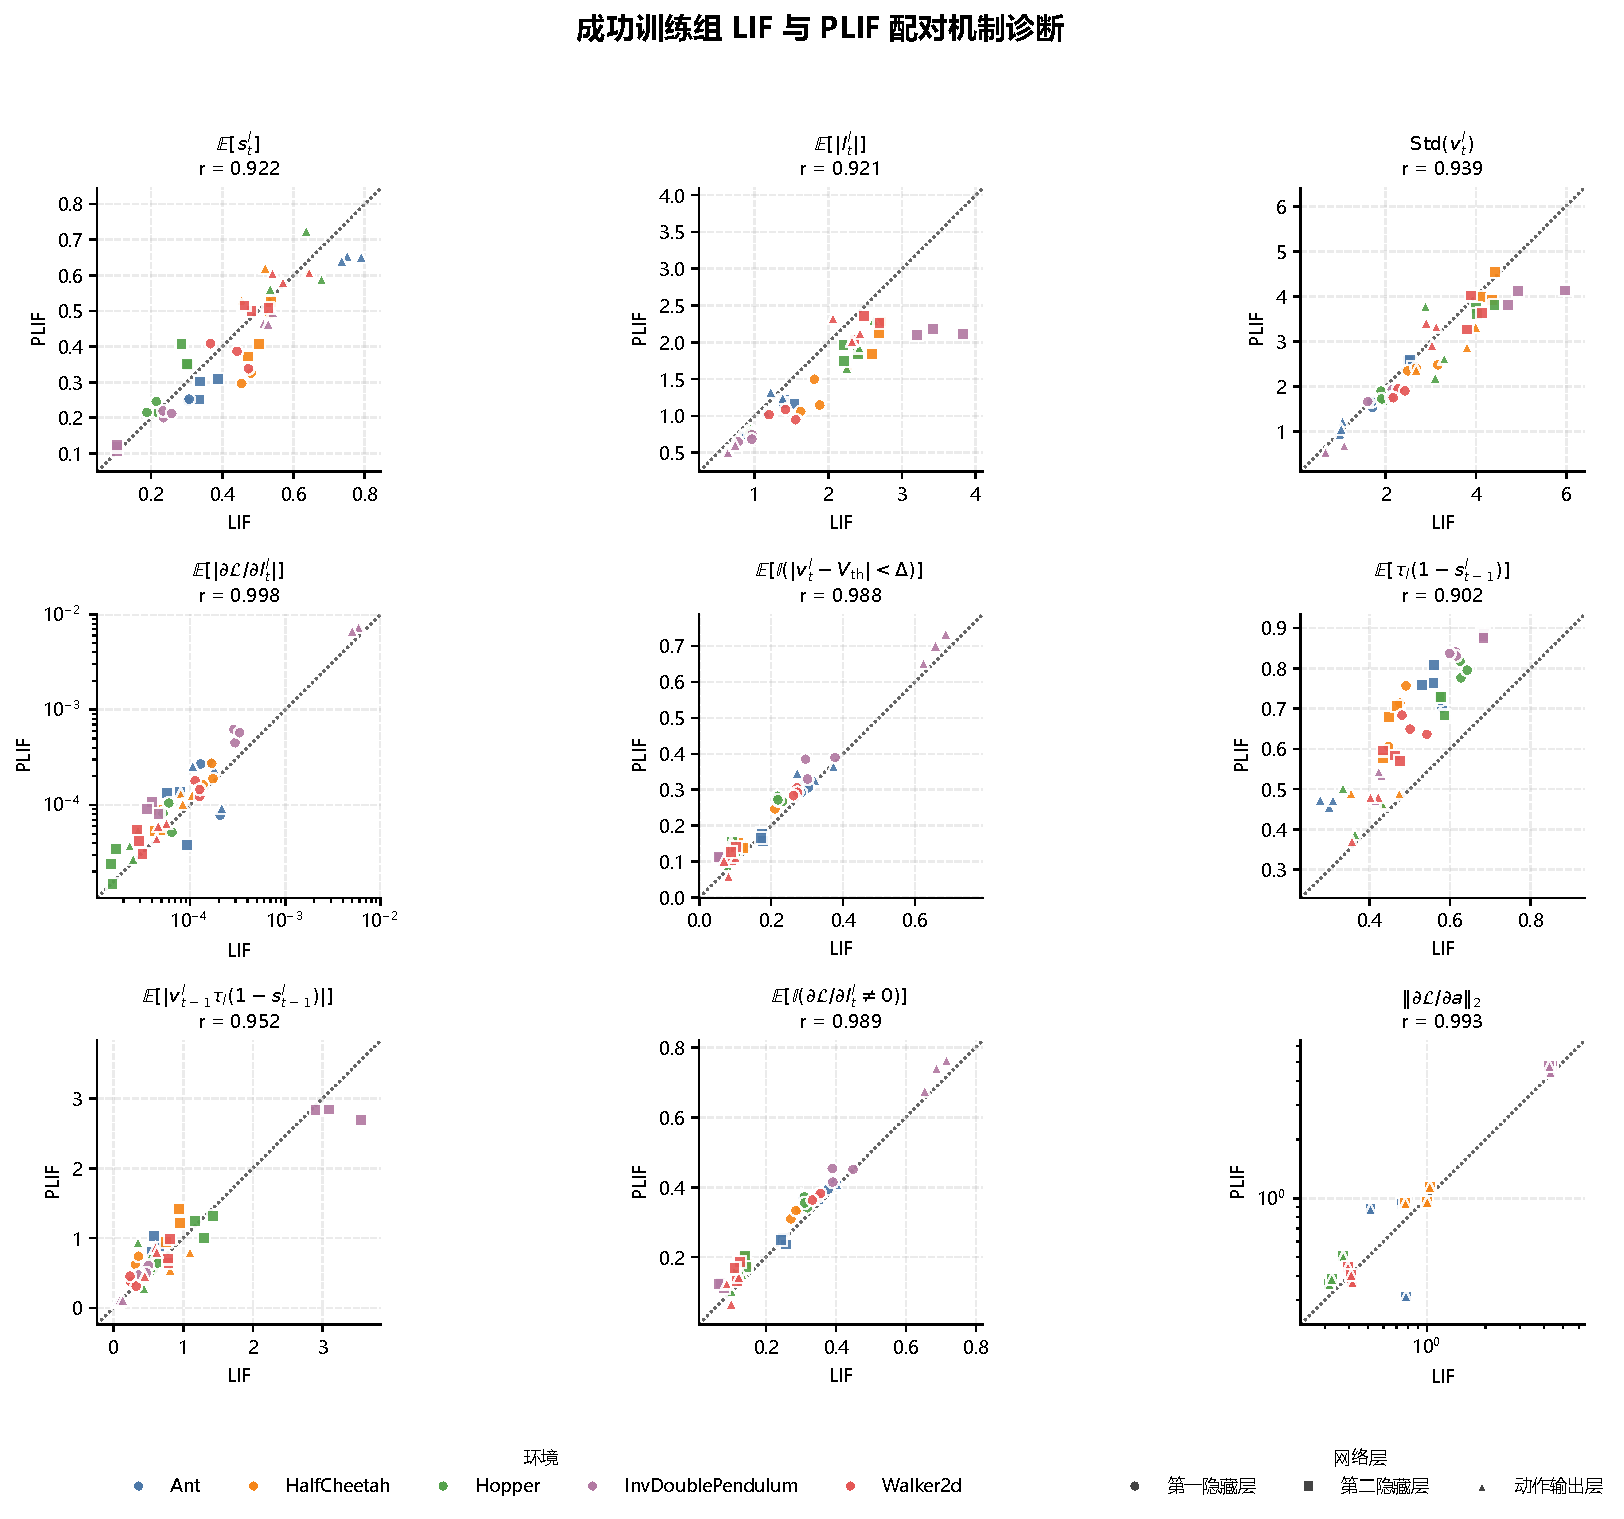
\includegraphics[width=\textwidth,height=0.82\textheight,keepaspectratio]{../../figures/lif_plif_success_mechanism_paired.pdf}
\caption{成功训练组中 LIF 与 PLIF 的配对机制诊断指标对比。每个点对应一个环境、随机种子和网络层在训练后期的平均值，虚线表示 $y=x$。较高的配对相关性说明二者在放电状态、膜电位尺度、代理梯度窗口占比和反向梯度通道上具有相近的训练机制。}
\label{fig:lif-plif-success-mechanism-paired}
\end{figure}

结果表明，LIF 与 PLIF 在多数机制指标上呈现较强一致性。后期放电率、电流幅值、膜电位标准差和电流梯度绝对值的配对相关系数分别为 $0.922$、$0.921$、$0.939$ 和 $0.998$，参数级权重梯度和偏置梯度的相关系数也分别达到 $0.943$ 和 $0.971$。进一步记录的代理梯度窗口占比、非零电流梯度占比、动作梯度范数和真实保留电压幅值相关系数分别为 $0.988$、$0.989$、$0.993$ 和 $0.952$，说明二者在前向放电、电流与膜电位尺度以及 STBP 反向传播通道上都保持了相似的层间和环境间结构。

值得注意的是，有效保留项在 PLIF 中整体高于 LIF，其相关系数为 $0.902$。这一现象与前文的时间常数分析一致：PLIF 通过可学习时间常数提高部分层的膜电位保留能力，但这种提高并未使放电模式、代理梯度窗口占比和梯度通道发生显著分化。换言之，PLIF 的额外自由度主要是在 LIF 已有机制附近进行连续调节，而不是使 actor 进入一套显著不同的训练动力学。

因此，本文将 LIF 与 PLIF 的关系表述为实验诊断意义上的机制近似等价。二者在神经元方程上并不完全相同，PLIF 仍然具有可学习时间常数这一额外自由度；但在当前 Proxy Target + TD3 框架和成功训练设置下，二者的任务回报、放电状态、膜电位尺度、代理梯度窗口占比、有效梯度覆盖率以及动作端梯度强度均呈现高度一致的配对结构。本文因此不将 PLIF 表述为全面优于 LIF 的替代模型，而将其理解为一种在相近成功训练机制中提供时间常数自适应能力的神经元模型。

\FloatBarrier

\chapter{总结与展望}

\section{全文工作总结}
脉冲神经网络具有事件驱动和稀疏计算等特点，在低功耗智能控制和神经形态硬件部署中具有潜在优势。将 SNN 引入连续控制强化学习时，actor 不仅需要输出连续动作，还需要在离散脉冲发放、膜电位递推和代理梯度反向传播之间保持稳定的训练动力学。Proxy Target 框架通过引入连续可微的代理目标网络，缓解了脉冲 actor 与 TD3 目标网络机制之间的不匹配问题，为 SNN actor 应用于连续控制任务提供了可行路径。在此基础上，本文围绕可学习膜电位时间常数是否能够改变 Proxy Target 脉冲强化学习的训练机制展开研究，重点比较 LIF 与 PLIF 脉冲 actor 的性能表现和内部训练状态。

本文首先介绍了强化学习、TD3、脉冲神经网络、LIF/PLIF 神经元、代理梯度和 STBP 等理论基础，并结合当前代码实现说明了 PLIF 脉冲 actor 的网络结构、时间常数参数化方式和训练流程。随后，本文在多个 MuJoCo 连续控制环境中整理 ANN、LIF、PLIF 和 CLIF 等方法的实验结果，并以最大评估回报和学习曲线作为总体性能分析入口。实验结果表明，PT-PLIF 与 PT-LIF 在当前实验范围内并没有表现出稳定、普适的性能优势差距，因此本文没有将 PLIF 表述为全面优于 LIF 的替代模型，而是进一步从训练机制角度分析脉冲 actor 为什么会出现低回报停滞。

在机制分析部分，本文以 Hopper-v4 中的 PLIF 失败组和 actor 更新间隔调整组作为代表案例，进一步考察 STBP 梯度传播、放电状态和 PLIF 时间常数演化之间的关系。分析表明，失败组并不是简单进入脉冲沉默状态，而是在前向传播仍保持较高放电率的同时，反向传播中的有效 STBP 梯度已经塌缩，导致权重、偏置和 PLIF 时间常数难以继续获得学习信号。相比之下，actor 更新间隔调整组在隐藏层保持更稀疏的放电状态，并持续保留非零梯度，使 actor 能够继续通过 critic 提供的策略损失更新参数。

此外，本文还结合 PLIF 时间常数的层间演化说明，可学习时间常数并不是在所有层上单调增大，而是表现出与网络功能相关的层间分化。隐藏层时间常数在成功组中明显增大，并与较低放电率共同提高有效膜电位保留能力；动作输出层则不必同步增大时间常数，而是更直接服务于动作 population 的读出。由此可见，PLIF 的主要价值不应被简单概括为最终回报提升，而应理解为为 SNN actor 提供了可分析的时间尺度自适应机制。本文的实验和分析共同说明，在 Proxy Target + TD3 框架下，脉冲 actor 的训练效果不仅取决于神经元模型本身，也受到放电状态、膜电位尺度、代理梯度窗口和 actor 更新频率等因素的共同影响。

在第五章最后，本文进一步补充了 LIF 与 PLIF 成功训练组的配对机制分析。该部分不再仅从最终回报判断二者优劣，而是比较放电率、电流幅值、膜电位分布、代理梯度窗口占比、有效保留项、非零电流梯度占比和动作梯度范数等内部诊断指标。结果显示，在当前 Proxy Target + TD3 框架和成功训练设置下，PT-LIF 与 PT-PLIF 在多数前向动力学和反向梯度指标上具有较高一致性。PLIF 的可学习时间常数确实增强了部分隐藏层的膜电位保留能力，但这种额外自由度并未使其形成与 LIF 完全不同的训练机制。因此，本文最终将二者关系概括为机制上的近似等价：PLIF 提供了更可解释的时间尺度调节能力，但并不必然带来稳定的最终性能优势。

从理论意义看，本文将 PLIF 的可学习时间常数放入完整的 Proxy Target + TD3 训练闭环中考察，说明该参数的作用必须依赖 STBP 梯度、放电重置和代理梯度窗口共同决定，而不能脱离训练动力学单独理解。该结论有助于把 LIF 与 PLIF 的比较从“最终回报优劣”推进到“时间尺度调节如何影响梯度路径”的机制层面。从应用价值看，本文整理的梯度、放电率、有效保留项和时间常数等诊断指标，可用于识别 SNN actor 中“前向仍放电、反向已失效”的训练停滞状态，并为 actor 更新频率、神经元时间常数和相关超参数的调节提供依据。因而，本文的结论不只是说明 PLIF 未稳定提升回报，也为后续构建更稳定、更可解释的低功耗连续控制脉冲 actor 提供了分析框架。

\section{主要研究结论}
综合前文实验与分析，本文得到以下几方面结论。

第一，PT-PLIF 与 PT-LIF 在当前实验范围内整体表现接近。虽然 PLIF 在神经元模型上比 LIF 多出可学习时间常数这一自由度，但从五个 MuJoCo 连续控制任务的最大评估回报和学习曲线看，二者并没有形成稳定、普适的性能差距。个别环境或随机种子中的优势不能直接推出 PLIF 全面优于 LIF。对连续控制强化学习而言，最终性能不仅由单个神经元模型决定，还受到 critic 学习、proxy target 拟合、actor 更新频率、探索噪声以及随机种子等因素共同影响。

第二，Hopper-v4 默认失败组揭示了一类“前向仍放电、反向已失效”的训练停滞模式。失败组后期并未进入脉冲沉默，隐藏层和动作输出层仍保持较高放电率；但由于电流幅值较大、膜电位分布更分散，同时频繁放电通过重置项削弱膜电位历史路径，STBP 有效梯度逐渐塌缩。此时 actor 虽然仍能产生动作，但权重、偏置和 PLIF 时间常数都难以继续获得有效学习信号，评估回报也长期停留在低水平。

第三，调整 actor 更新频率能够在代表性案例中缓解上述失败模式。以随机种子 10991 的单腿跳跃任务为例，默认 \texttt{policy\_freq}=2 配置稳定停留在低回报区间；将 actor 更新间隔调整为 \texttt{policy\_freq}=4 后，训练能够进入高回报区间。诊断结果表明，成功组的隐藏层放电更稀疏，电流和膜电位尺度更接近代理梯度有效区域，并且在训练后期仍能保持非零 STBP 梯度。该结果说明，训练稳定性不仅取决于神经元是否可学习，还与 actor 更新节奏和反向梯度通道是否保持健康密切相关。

第四，PLIF 时间常数呈现具有功能差异的层间演化。成功训练中，隐藏层时间常数倾向于增大，并与较低放电率共同提高未放电路径上的有效膜电位保留项；动作输出层时间常数则不一定同步增大，甚至可能下降到低于初始值。这说明 PLIF 并不是简单地在所有层延长记忆，而是根据不同层在表示学习和动作读出中的作用形成差异化调节。隐藏层更需要保留亚阈值历史信息，输出层则更直接服务于动作 population 的即时读出。

第五，LIF 与 PLIF 在成功训练状态下具有机制近似等价性。配对诊断结果显示，二者在后期放电率、电流幅值、膜电位尺度、代理梯度窗口占比、非零电流梯度占比和动作梯度范数等指标上保持高度一致。PLIF 的有效保留项整体高于 LIF，说明其额外时间常数确实发挥了调节作用；但这种调节主要发生在 LIF 已有训练机制附近，并没有改变 Proxy Target 脉冲 actor 的基本学习路径。因此，PLIF 更适合作为分析 SNN actor 时间尺度自适应的工具，而不是被表述为必然提高最终回报上限的替代模型。

总体而言，本文结论的理论价值在于明确了可学习时间常数、放电重置和代理梯度传播之间的耦合关系，避免将 PLIF 简化理解为单纯提升性能的神经元替换项；其应用价值在于给出一组可操作的训练状态诊断指标和调参依据，为后续在连续控制任务中训练稳定、可解释并具备低功耗潜力的 SNN actor 提供参考。

\section{研究不足}
尽管本文围绕 Proxy Target 框架下 LIF 与 PLIF 脉冲 actor 的训练机制进行了较为细致的实验分析，但仍存在一些不足。

首先，实验覆盖范围仍有进一步扩展空间。本文主要使用五个 MuJoCo 连续控制环境和有限数量随机种子进行比较，能够支持当前范围内的机制分析，但还不足以穷尽所有连续控制任务、网络规模和训练难度。尤其是在强化学习中，不同随机种子、环境版本、探索噪声和评估方式都可能带来较大波动，因此本文结论更适合表述为当前实验条件下的观察，而不是所有场景中的普遍定理。

其次，失败机制分析主要围绕 Hopper-v4 的代表性案例展开。该环境能够清楚展示“仍然放电但梯度塌缩”的现象，也便于对失败组和成功组进行对照；但相同现象在其他环境中的出现概率、触发条件和缓解方式仍需要更多系统实验支撑。本文中的重复运行主要用于说明同一设置下机制现象可以复现，而不是严格意义上的跨随机种子统计显著性检验。

再次，本文尚未对 \texttt{proxy\_lr}、\texttt{policy\_freq}、actor 学习率、PLIF 时间常数学习率等超参数之间的交互关系进行完整网格化分析。当前结果能够说明在代表性设置中调整 actor 更新间隔可以缓解失败模式，但还不能进一步断言某一个超参数在所有任务上具有单独、稳定且可泛化的因果作用。未来仍需要更系统的消融实验区分 proxy target 拟合速度、actor 更新频率和脉冲神经元参数更新之间的耦合关系。

最后，本文主要关注训练机制和回报表现，对脉冲 actor 的能耗优势和硬件部署价值尚未进行直接评估。SNN 的重要潜力来自事件驱动计算、稀疏放电和神经形态硬件适配，但本文尚未系统统计实际推理过程中的脉冲率、稀疏性、延迟、显存占用和硬件能耗。因此，本文对“低功耗智能控制”的讨论仍主要停留在方法潜力和训练机制层面，尚未形成完整的部署评估闭环。

\section{未来展望}
针对上述不足，后续工作可以从以下几个方向继续推进。

第一，可以扩展实验任务和随机种子数量，进一步检验 LIF 与 PLIF 近似等价结论的稳健性。除本文使用的 MuJoCo 任务外，还可以引入更复杂的机器人控制环境、不同动力学难度的任务以及更长训练步数设置，观察 PLIF 时间常数自适应是否会在更长时序依赖或更高维动作空间中表现出更明显作用。同时，增加随机种子和重复运行次数，有助于区分稳定机制现象与偶然训练波动。

第二，可以系统研究 Proxy Target 训练超参数对脉冲 actor 稳定性的影响。未来可围绕 \texttt{proxy\_lr}、\texttt{policy\_freq}、proxy 更新次数、actor 学习率和 PLIF 时间常数学习率设计更完整的消融实验，并结合 STBP 梯度、代理梯度窗口占比和参数统计量建立训练状态判据。这样不仅可以解释某一组配置为什么成功或失败，也可能为 Proxy Target + SNN actor 提供更可操作的超参数选择原则。

第三，可以进一步完善 LIF 与 PLIF 的机制对照框架。本文已经从成功训练状态说明二者在多数诊断指标上高度接近，后续还可以补充更多失败组、临界组和不同时间阶段的配对分析，观察二者在训练早期、中期和后期是否始终保持相似结构。若能将放电状态、膜电位分布、代理梯度窗口和时间常数演化统一到同一诊断框架中，将有助于更准确地判断 PLIF 额外自由度何时有效、何时被整体训练动力学所限制。

第四，可以将研究从训练机制进一步推进到部署效率评估。未来可在相同控制性能下比较 ANN、LIF、PLIF 和其他 SNN actor 的平均放电率、事件稀疏性、推理延迟和理论能耗，并探索在 Loihi 等神经形态硬件或事件驱动推理平台上的实现方式。只有将训练稳定性、任务回报和硬件效率共同纳入评价，才能更完整地判断脉冲强化学习方法在实际智能控制任务中的应用价值。

\backmatter
\ctexset{chapter={format=\centering\heiti\zihao{-3}\bfseries}}
\begin{thebibliography}{99}
\addcontentsline{toc}{chapter}{参考文献}
\bibitem{sutton2018rl}
Sutton R S, Barto A G. Reinforcement Learning: An Introduction[M]. 2nd ed. Cambridge, MA: MIT Press, 2018.

\bibitem{lillicrap2016ddpg}
Lillicrap T P, Hunt J J, Pritzel A, et al. Continuous Control with Deep Reinforcement Learning[C]//Proceedings of the 4th International Conference on Learning Representations. San Juan, Puerto Rico: OpenReview.net, 2016.

\bibitem{fujimoto2018td3}
Fujimoto S, van Hoof H, Meger D. Addressing Function Approximation Error in Actor-Critic Methods[C]//Proceedings of the 35th International Conference on Machine Learning. Stockholm, Sweden: PMLR, 2018: 1587-1596.

\bibitem{haarnoja2018sac}
Haarnoja T, Zhou A, Abbeel P, Levine S. Soft Actor-Critic: Off-Policy Maximum Entropy Deep Reinforcement Learning with a Stochastic Actor[C]//Proceedings of the 35th International Conference on Machine Learning. Stockholm, Sweden: PMLR, 2018: 1861-1870.

\bibitem{todorov2012mujoco}
Todorov E, Erez T, Tassa Y. MuJoCo: A Physics Engine for Model-Based Control[C]//2012 IEEE/RSJ International Conference on Intelligent Robots and Systems. Vilamoura-Algarve, Portugal: IEEE, 2012: 5026-5033.

\bibitem{davies2018loihi}
Davies M, Srinivasa N, Lin T H, et al. Loihi: A Neuromorphic Manycore Processor with On-Chip Learning[J]. IEEE Micro, 2018, 38(1): 82-99.

\bibitem{wu2018stbp}
Wu Y, Deng L, Li G, Zhu J, Shi L. Spatio-Temporal Backpropagation for Training High-Performance Spiking Neural Networks[J]. Frontiers in Neuroscience, 2018, 12: 331.

\bibitem{lee2016backprop}
Lee J H, Delbruck T, Pfeiffer M. Training Deep Spiking Neural Networks Using Backpropagation[J]. Frontiers in Neuroscience, 2016, 10: 508.

\bibitem{zenke2018superspike}
Zenke F, Ganguli S. SuperSpike: Supervised Learning in Multilayer Spiking Neural Networks[J]. Neural Computation, 2018, 30(6): 1514-1541.

\bibitem{shrestha2018slayer}
Shrestha S B, Orchard G. SLAYER: Spike Layer Error Reassignment in Time[C]//Advances in Neural Information Processing Systems 31. Montréal, Canada: Curran Associates, 2018: 1419-1428.

\bibitem{neftci2019surrogate}
Neftci E O, Mostafa H, Zenke F. Surrogate Gradient Learning in Spiking Neural Networks: Bringing the Power of Gradient-Based Optimization to Spiking Neural Networks[J]. IEEE Signal Processing Magazine, 2019, 36(6): 51-63.

\bibitem{tang2020popsan}
Tang G, Kumar N, Yoo R, Michmizos K P. Deep Reinforcement Learning with Population-Coded Spiking Neural Network for Continuous Control[C]//Proceedings of the 4th Conference on Robot Learning. Cambridge, MA: PMLR, 2021: 2016-2029.

\bibitem{fang2021plif}
Fang W, Yu Z, Chen Y, et al. Incorporating Learnable Membrane Time Constant to Enhance Learning of Spiking Neural Networks[C]//Proceedings of the IEEE/CVF International Conference on Computer Vision. Montréal, Canada: IEEE, 2021: 2661-2671.

\bibitem{bellec2018lsnn}
Bellec G, Salaj D, Subramoney A, et al. Long Short-Term Memory and Learning-to-Learn in Networks of Spiking Neurons[C]//Advances in Neural Information Processing Systems 31. Montréal, Canada: Curran Associates, 2018: 795-805.

\bibitem{zhang2022mdc}
Zhang D, Zhang T, Jia S, Xu B. Multi-Sacle Dynamic Coding Improved Spiking Actor Network for Reinforcement Learning[C]//Proceedings of the AAAI Conference on Artificial Intelligence. Palo Alto, CA: AAAI Press, 2022, 36(1): 59-67.

\bibitem{chen2024fully}
Chen D, Peng P, Huang T, Tian Y. Fully Spiking Actor Network with Intra-layer Connections for Reinforcement Learning[J]. IEEE Transactions on Neural Networks and Learning Systems, 2025, 36(2): 2881-2893.

\bibitem{xu2025proxy}
Xu Z, Bu T, Hao Z, Ding J, Yu Z. Proxy Target: Bridging the Gap Between Discrete Spiking Neural Networks and Continuous Control[C]//Proceedings of the 39th Conference on Neural Information Processing Systems. San Diego, CA: Curran Associates, 2025.
\end{thebibliography}

\ctexset{chapter={format=\centering\heiti\zihao{-3}\bfseries}}
\chapter*{致谢}
\addcontentsline{toc}{chapter}{致谢}

本科阶段的学习与本论文的完成，离不开许多师长、同学和家人的帮助与支持。在论文即将完成之际，谨向所有关心和帮助过我的人致以诚挚的感谢。

首先，衷心感谢我的指导教师于强老师。在论文选题、研究思路梳理、实验方案设计以及论文写作过程中，老师给予了我耐心细致的指导。老师严谨的治学态度、清晰的问题意识和务实的科研作风，使我在完成毕业论文的过程中不仅加深了对类脑神经网络与强化学习相关问题的理解，也逐渐学习到如何从实验现象中提炼问题、分析机制并形成较为完整的研究表达。

其次，感谢在课题推进过程中给予我具体指导和帮助的学长。无论是在代码实现、实验配置、结果整理，还是在论文结构和表述细节上，学长都给予了我许多宝贵建议。这些帮助使我能够更顺利地理解已有工作、定位实验问题，并不断完善本文的研究内容。

最后，感谢我的父母一直以来的理解、支持与陪伴。正是他们在生活和精神上的鼓励，使我能够安心完成本科阶段的学习与毕业论文工作。未来我也将带着这份支持继续前行，努力以更加踏实的态度面对新的学习和工作。

\end{document}
